\documentclass{article}
\usepackage[utf8]{inputenc}
\usepackage{amsmath}

%%%%% ADDED BY TOMMY %%%%%
\usepackage{xcolor}
\usepackage{xspace}
\usepackage{amsfonts}
\usepackage{graphicx}
\usepackage{booktabs}
\usepackage{hyperref}
\DeclareMathOperator*{\argmin}{arg\,min}
\DeclareMathOperator*{\argmax}{arg\,max}

\newcommand{\Ie}{\textit{I.e.}\xspace}
\newcommand{\ie}{\textit{i.e.}\xspace}
\newcommand{\Eg}{\textit{E.g.}\xspace}
\newcommand{\eg}{\textit{e.g.}\xspace}
\newcommand{\probP}{\text{I\kern-0.15em P}}

\DeclareMathOperator*{\minimise}{\textrm{minimise}}
\DeclareMathOperator*{\maximise}{\textrm{maximise}}

\newcommand{\tl}[1]{\textit{[{\color{red}#1}]}}
\newcommand{\cm}[1]{\textit{[{\color{blue}#1}]}}

\newcommand{\erik}[1]{\textit{[{\color{brown}Erik: #1}]}}
% \newcommand{\erik}[1]{}
%%%%%%%%%%%%%%%%%%%%%%%%%%

% \usepackage{itemize}
\title{Safety-critical computer vision: A survey of adversarial evasion attacks and defenses on computer vision systems}
\author{Charles Meyers}
%TODO add other authors and emails


\begin{document}

\maketitle
\begin{abstract}

Considering the growing prominence of production-level AI and the threat of adversarial attacks that can poison a model against a certain label, evade classification, or reveal sensitive data about the model and training data to an attacker, adversaries pose fundamental problems to machine learning systems.

While many defenses have been proposed, they are often computationally expensive and tend to reduce model accuracy. Furthermore, recent research has shown that most defenses have worse performance against adversaries not tested at the time of publishing, arising from the tendency to only publish the `best' results. Additionally, increased hardware capacity means that subsequent researchers are able to perform larger analyses in the same amount of time.
% \erik{Do we believe there is any aspect of defences being "too" tailored to the adversaries used for development and testing and hence not as "generalizable" as one would hope and claim them to be?}
% \cm{I would say this is clear from the Madry 2017 paper that L2 defenses don't generalize to L1 attacks and vice versa. This makes some kind of sense because I can construct an L0 attack that of radius = 1 that flips the most significant bit, but this would likely violate the distance constraints when applied to a different metric. However, I think we should be just as worried about single-pixel attacks as we are about small perturbation attacks across the entire image. This problem, however, is largely ignored/side-stepped in papers like CCAT which compare L1 attacks to L1 defenses. I had tried to show that CCAT doesn't generalize in the SVM paper, but that was misread as showing that \textbf{my} technique didn't work, not that the CCAT authors presented something that does not generalize. How I present this is probably still somewhat of an open question because I do think people are aware of this, but admitting that your fancy new defense doesn't generalize is not something people write in their papers.}

This published optimism poses a particular problem for real-time and safety-critical systems, governed by legal constraints, in which software changes must be explainable, every change must be thoroughly tested, and verifying a change currently means testing against millions or billions of samples. Even worse, there is a growing body of research that suggests accuracy and robustness are inversely related---implying that better models simply lead to better adversaries, raising fundamental questions about the robustness potential of high-dimensional neural network architectures and/or high-dimensional data.

We have therefore conducted a large survey of attacks and defenses that spans the short history of the adversarial robustness field. We present a simple and practical framework for analyzing any machine-learning system from a safety-critical perspective and use this to conclude that all tested configurations of the ResNet architecture fail to meet any reasonable definition of `safety-critical' when tested on even small-scale benchmark data.

% \erik{I assume this not to be the best to do but bring up the alternative anyway... One could, alternatively, make the framework a more highlighted contribution by start telling about the framework and then tell that it has been used to analyze a large set of methods. (If going for the latter, one should also modify the title. (But I guess the framework is not so strong of a contribution.)}

In this study, we examine myriad state of the art defenses and attacks against computer vision systems with a focus on safety-critical applications in autonomous driving, industrial control, and healthcare. By testing a combination of attacks and defenses, their efficacy, and their run-time requirements, we provide substantial empirical evidence that modern neural networks consistently fail to meet established safety-critical standards by a wide margin.

% We evaluate a large suite of proposed attacks and defenses in the contexts of accuracy, worst-case failure rate, and computation time.  We provide substantial empirical evidence that an attacker has a fundamental advantage when it comes to computational cost as accuracy scales with $\mathcal{O}(1/\sqrt{n})$~\cite{vapnik1994measuring}, where $n$ is the number of samples, but that an attacker can break a model in a small number ($\leq 10$) of iterations on a dataset that was otherwise unknown during training. We show that every model defense configuration reduces the \textit{accuracy} on benign (unperturbed) data. We show that, even when a particular defense improves the \textit{failure rate} against a given attack, that that behavior is inconsistent across metric spaces and attack types. Most importantly, we conclude that each and every tested configuration fails to meet safety-critical standards by a wide margin.

\end{abstract}





\section{Introduction}

\paragraph{Motivation.}

Vehicular accidents, medical mistakes, and industrial safety failures are among the leading causes of preventable death around the world~\cite{OECD, makary2016medical, icoh}. Technologies like image classification systems have shown to be more accurate than their human counterparts under strict laboratory conditions in these domains~\cite{nhtsa, pakdemirli2019artificial, bernal2017safety++}. However, prior research has shown that machine learning systems often fail to correctly classify images after small perturbations to the original image. While these ``adversarial attacks''~\cite{chakraborty_adversarial_2018, biggio_evasion_2013-1}, define a worst-case scenario for a given data pipeline, imperfect data is a natural result of any sufficiently complex system~\cite{pearson2005mining}. In this work, we focus on intentional perturbations to the input space where the goal is to~\emph{evade} a classifier, but similar perturbations are a natural consequence of modern neural network architectures and hardware setups (see Section \ref{classification}). Prior research has shown that proper data sanitation, anomaly detection, and model retraining are effective ways to combat adversarial attacks~\cite{chakraborty_adversarial_2018, shirazi_survey_nodate, grigorescu2020survey}. However, even state of the art defenses reduce the failure rate when compared to the un-defended (control) model, suggesting that the actual ability to generalize beyond laboratory test cases has been overestimated in the literature which has been noted before by Croce~\cite{croce_reliable_2020}, for example, and we confirm below (see Section~\ref{results}).

% \erik{Our focus is on evasion attacks - but would it in a survey make sense to put that even more into context by in short (somewhere in the paper) presenting not only what we focus on but what are the other types, not in focus of this paper?}

Further questions about the feasibility of truly `safe' artificial intelligence (AI) have been raised. For instance, it has been proven that no matter where we draw our boundary conditions, there exists an attack that will confuse any (non-perfect) discriminator or shift its boundary conditions~\cite{dohmatob_generalized_2019}. Additionally, while attacks are always possible on paper, a cost-aware analysis can reveal the feasibility of such attacks in practice. It is critical for any safety-critical system to be robust to these attacks because, as we demonstrate, wide classes of attacks are cost-effective even when we restrict perturbations to a single byte (see Section~\ref{fig:grid}).

% TODO: rephrase this with above abstract text

We evaluate a large suite of proposed attacks and defenses in the contexts of accuracy, worst-case failure rate, and computation time.   We show that every model defense configuration reduces the \textit{accuracy} on benign (unperturbed) data. We show that, even when a particular defense improves the \textit{failure rate} against a given attack, that that behavior is inconsistent across distance measures and attack types. Most importantly, we conclude that each and every tested configuration fails to meet safety-critical standards by a wide margin.


% We provide substantial empirical evidence that an attacker has a fundamental advantage when it comes to computational cost as the training accuracy scales with $\mathcal{O}(1/\sqrt{n})$~\cite{vapnik1994measuring}, where $n$ is the number of samples, but that an attacker can break a model in a small number ($\leq 10$) of iterations on a dataset that was otherwise unknown during training.\textbf{}



\paragraph{Contributions.} 
Our contributions can be summarized as follows.

\begin{itemize}
    \item We show that even state-of-the-art defenses fail at making models that meet safety critical standards even if they tend to marginally improve the failure rate.
    \item We survey a wide variety of defenses on standard datasets and provide a novel evaluation criterion for examining model failure-rate in the context of safety-critical systems.
    \item We apply time and cost analysis for both the attacks and the defenses, something rarely done in the literature.
    \item We provide new insight into the robustness versus accuracy problem.
    \item We establish a standards-based framework for testing safety-critical computer vision systems in a way that meets regulatory standards without needing a burdensome number of test images.
    \item We survey a large suite of attacks and defenses to examine how each defense fares against each attack, measuring accuracy, worst-case failure rate, and run-time requirements.
\end{itemize}





\section{Background}

Machine learning, artificial intelligence, and automated data collection are increasingly used in safety-critical applications like autonomous vehicles~\cite{grigorescu2020survey, al2017deep}, medical imaging~\cite{ching2017opportunities, sahiner2019deep}, and industrial control~\cite{fukuda1992theory, monmasson2011fpgas}. Convolutional neural networks (CNNs) have demonstrated unparalleled accuracy in image classification tasks; however, CNNs have been shown to be very fragile to adversarial attacks~\cite{miller_adversarial_2020, finlayson2018adversarial}.  Research points to societal trust in fully automated banking thanks to, among other things, verifiable transactions and guarantees from the issuing institution~\cite{safetyframework}. However, when it comes to real-time, safety-critical deep learning, models are rarely reproducible or verifiable~\cite{tsipras_robustness_2019, carlini_towards_2017}. Despite the drawbacks of deep-learning, modern aviation relies on an array of sensors to make largely automated decisions, relying on a framework of component testing and simulation~\cite{aviation}. While similar test suites for adversarial robustness have been proposed~\cite{carlini_towards_2017, chakraborty_adversarial_2018}, they rely on \textit{de facto} accuracy goals rather than a solid theoretical and legal framework. Below we propose such a framework.


% The lack of empirical examples highlights either systemic overfitting as demonstrated by \cite{paper_about_reproducibility} and the lack of a generalized robustness theory.


\paragraph{Safety Critical Automation.}

\label{safety-critical}
Since the bulk of the literature focuses on image classification systems~\cite{dohmatob_generalized_2019, biggio_evasion_2013-1, bect_bayesian_2017, chakraborty_adversarial_2018, carlini_towards_2017, croce_reliable_2020}, we chose to stress test them in the contexts of autonomous vehicles, medical imaging, and industrial control which are each governed by pre-existing standards across the different domains. Safety-critical software is already widely deployed in other electro-mechanical systems like vehicular braking systems~\cite{braking}, aviation~\cite{aviation}, and medical implants (\eg, pacemakers)~\cite{tuan2010modeling}. The International Standards Organization provides a safety-threshold of $10^{-9}$ failures per hour for any life-threatening situation~\cite{iso26262} and $10^{-6}$ for any risk of harm, required of any automotive or aviation system governed by ISO~26262~\cite{iso26262}. For an autonomous vehicle trying to classify objects on the road, a false negative classification of, say, a cyclist could lead to death, whereas false positive detection of a cyclist would be more likely to cause braking-related injuries that are less severe corresponding to the legal and technical requirements outlined in these international standards. This would be a requirement for any system intended to aid in trajectory planning. Whether the component be hardware or software, each component must meet the requirement in isolation, raising questions of legal compliance for any system that relies on proxy models, attack detection, or any other type of out-of-band component to ensure safety. For medical imaging, a false negative classification could mean loss of life whereas a false positive is less likely to cause grievous harm (but likely to be lead to expensive and unnecessary additional testing)  Electro-industrial safety systems are generally governed by the International Electrotechnical Commission, IEC~61508~\cite{IEC61508}\tl{Reference broken.} and medical software in particular requires continuous failure rate testing adding a massive computational burden to the development phase as governed by IEC~62034~\cite{IEC 62304}\tl{Reference broken.}. In general, acceptable risk is expressed as a matrix (see Table~\ref{tab:rate}) where these classes are known in the standard as the safety integrity level (SIL). Which then corresponds to different failure modes for components that act on-demand (\eg, medical imaging) or ones that act continuously (\eg, object detection in autonomous cars). SIL I failure rates are never acceptable, SIL II rates are only acceptable if mitigation is creates 

The failure rate is normally defined in the context of accuracy, such that:
\begin{equation}\label{eq:accuracy} 
    \mathrm{Failure~rate} = 1 - \mathrm{Accuracy} = 1 - \frac{\mathrm{True~Classifications}}{\mathrm{Total}},
\end{equation}
where \textit{Total} is the number of tested samples and \textit{True Classifications} refers to the number of objects that were correctly categorized by a given model. However, due to the order of magnitude of regulatory requirements and the strict commit-testing requirements for safety critical devices, these evaluations become an infeasible way to verify that a model only fails once across the required number of samples (see Table \ref{tab:rate}). Instead, we calculate failure rate as a function of time, using various attacks as a stand-in for the `worst-case' or upper-bound of the failure rate:
\begin{equation}\label{eq:failure_rate}
    \mathrm{Worst~case~failure~rate} = \frac{\mathrm{False~Classifications}}{\Delta t},
\end{equation}
where \textit{False~Classifications} is the number of misclassified samples and $\Delta t$ is the time taken to evaluate said samples.

\begin{table}[!h]
    \begin{center}
        \begin{tabular}{l cc cc}
            \toprule
            SIL & Keyword && On-demand Operation   & Continuous Operation \\
            \cmidrule{1-2} \cmidrule{4-5}
            I   & Unacceptable   && $[10^{-6}, 10^{-5})$  & $[10^{-10}, 10^{-9})$ \\
            II  & Undesirable  && $[10^{-7}, 10^{-6})$  & $[10^{-11}, 10^{-10})$ \\
            III & Tolerable  && $[10^{-8}, 10^{-7})$  & $[10^{-12}, 10^{-11})$ \\
            IV  & Acceptable  && $[10^{-9}, 10^{-8})$  & $[10^{-13}, 10^{-12})$ \\
            \bottomrule
        \end{tabular}
        \caption{Acceptable Failure Rates for different SIL levels in which a single death is possible, measured in failures per second.}
        \label{tab:rate}
    \end{center}
\end{table}




% \begin{table}[!h]
% \begin{center}
% \tiny
% \begin{tabular}{l c llll}
%     \toprule
%                  && \multicolumn{4}{c}{Consequence} \\
%     Failure Rate && Multiple Deaths & Single Death & Major Injury & Minor Injury \\
%     \cmidrule{1-1} \cmidrule{3-6}
%     Many times in a lifetime
%         && I         & I         & I         & II \\
%     Several times in a lifetime
%         && I         & I         & II        & III \\
%     Once in a lifetime
%         && I         & II        & III       & III \\
%     Unlikely in a lifetime
%         && II        & III       & III       & IV \\
%     Very unlikely in a lifetime
%         && III       & III       & IV        & IV \\
%     Incredibly unlikely in a lifetime
%         && IV        & IV        & IV        & IV \\
%     \bottomrule
% \end{tabular}
% \caption{SIL to Plain English mapping. I is never acceptable. We aim for IV.}
% \label{tab:sil}
% \end{center}
% \end{table}


In each evaluation, we measure both the failure rate typical in the literature (\eg, accuracy) as well as the worst-case failure rate. Further details can be found in Section~\ref{methods}. We examine attacks across several different distance metrics and contexts (Section:~\ref{attacks}) against many defenses (Section~\ref{defenses}).


\paragraph{Image Classification Systems.}
\label{classification}

In general, an image classification system, $K$, attempts to parse some image input signal, $x$, and output one of $k$ class labels, $\hat{y} = K(x)$, with $\hat{y} \in \{1,\ldots,k\}$. Each image is represented as a multi-dimensional array of $n\times m$ pixels, with bit depth $b$ and color depth $c$, such that they are of size $\frac{m \cdot n \cdot b \cdot c}{8}$ bytes. When the model is a neural network, the images are passed into a composition of `layers', each layer typically performing an affine transformation followed by a non-linear element-wise transformation (called an activation function). The parameters of such a composition of layers (called an `architecture') are found by minimizing a loss function, $L(\cdot,\cdot)$, that penalises differences between a true label, $y$, and an estimate, $\hat{y}$. When the problem is a multi-class classification, the loss function could, for instance, be the categorical cross-entropy loss~\cite{biggio_evasion_2013, tsipras_robustness_2019, croce_reliable_2020, carlini_towards_2017}.



% \paragraph{Bernoulli Schemes and Generalization}

% \cm{This makes sense in the topology paper. I'm not sure it's relevant to the discussion of safety-criticality.}
% \tl{I agree to remove this. I don't understand what you want to say with it? Perhaps if you make that more clear, it would make more sense to include it?}
%  If we assume that our classifier is not perfect, then we can model the probability mass function of the classifiers ability to correctly classify an image as
% $$
%     \probP(p, n, s) = \binom{n}{s} p^s (1-p)^{n-s} \Rightarrow \frac{n!}{s!(n-s)!} p^s(1-p)^{n-s},
% $$
% where $p$ is the probability of successful classification ($\mathbf{E} [K(x_i):\hat{y} - y] \forall x_i \in X$ in the standard statistics notation), $n$ is the number of trials, and $s$ is the number of successes~\cite{stats_textbook}. For multi-class classification systems, this notion of success is ambiguous since the `total population' of a multi-class set is ill-defined for a given class. As such, we have examined this in the context of both false negative and false positives (using recall and precision metrics respectively). 

% If we assume a fixed number of trials and $s = n-1$ successes, then $P$\tl{The $P$ is not defined.} becomes 
% $$
%     \probP(n, p) = \frac{n!}{(n-1)!} p^s (1-p) \Rightarrow np^{n-1}(1-p).
% $$

% %A number of these trials, $t$, with $\{p_i,\ldots,p_t\} \in P$ in succession is called a `Bernoulli Process' which generalizes to a `Bernoulli scheme' when expanded to experiments conducted on non-binary classes~\cite{topologytextbook} such that $[\bar{p_j},\ldots,\bar{p_k}] \forall [\bar{p_i},\ldots,\bar{p_t}] \in P$.

% The entropy, or uncertainty ($H$), in the system can be expressed as~\cite{shannon1948}
% $$
%     H(\probP) = - \sum_{i = 1}^t \sum_{j = 1}^k p_{ij} \log p_{ij}
% $$

% Cross-entropy loss, the standard loss function for multi-class classification problems is:

% $$
%     L_{H_{cross}} = - \sum_{x \in X} p(x) \log q(x)
% $$
% where $p$ and $q$ are the probabilities of success for the two probability mass functions you wish to compare. A deep learning model attempts to minimize this loss by changing the model weights between iterations while an attack seeks to maximize this using various strategies, each outlined respectively in \ref{defenses} and \ref{attacks}.



% A related measure, a formal measure of robustness \cite{hopskipjump}, Kullback Leibler divergence $D_{KL}$ is defined as

% $$
% D_{KL} = \sum{p(x) \frac{\log p(x)}{q(x)}}
% $$

% which captures the difference in output entropy between benign examples and their adversarial counterparts. Ideally, this would be 0, indicating no difference in performance between sets of benign and adversarial examples. That is, when $D_{KL} = 0$, the model can be considered robust against the set of attacks described by $q(x)$

\paragraph{Robustness.}
% \erik{Is this where you could gain some pedagogical point by the type of drawings you have showed a couple of times? (Without spending too much space.)}
% TODO: insert hyper-sphere graphic


% % Noisy Number
\begin{figure}[]
    {\centering
    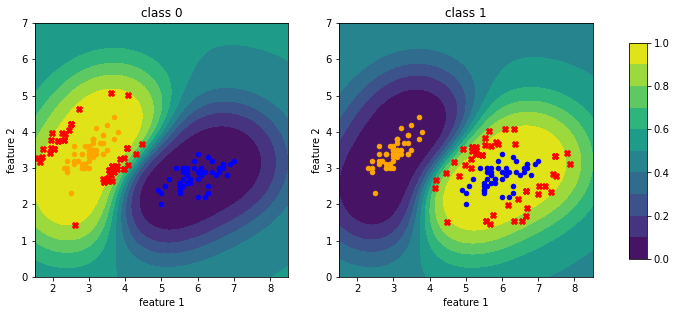
\includegraphics[width=.7\textwidth]{images/attacks.png}
    
    \caption{Orange (class 0) points, blue (class 1) points, and red (adversarial) points in a contour map for a radial basis function support vector classifier. The contours reflect the confidence levels for a given sample and class.}
    \label{fig:shift}
    } % end centering
\end{figure}


% % Attack Example
\begin{figure}[]
    {\centering
    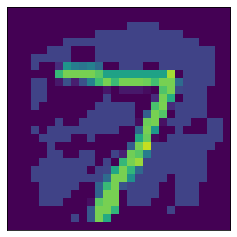
\includegraphics[width=.25\textwidth]{images/noisy_number.png}
    \caption{A `7' perturbed with adversarial noise such that the model in question detects it to be a `9.'}
    \label{fig:attack}
    } % end centering
\end{figure}

In general, an \textit{attacker} seeks to maximize loss against a given model rather than to minimize it. This is accomplished by perturbing samples from one class so that they fall within the highly confident region of another, incorrect class. Figure \ref{fig:shift} depicts a radial basis function support vector machine, classifying the points into orange (class 0) or blue (class 1). However, the red indicates successfully generated adversarial examples. Figure \ref{fig:attack} shows an example of a `7' that has added adversarial noise such that the classifier sees it to be a `9'. 
In related surveys~\cite{dohmatob_generalized_2019, biggio_evasion_2013-1, bect_bayesian_2017, chakraborty_adversarial_2018, carlini_towards_2017, croce_reliable_2020}, a model's adversarial robustness is defined as its performance accuracy against a given adversary. A thorough examination of such attacks are explored in Section~\ref{attacks} below, but, in general, an attacker perturbs an image such that the perturbation distance, $d$, is less than or equal to a threshold value, $\epsilon$, specified by the experimenter, under some conception of distance. The evaluations in this study examine both the $\ell_{\infty}$ and $\ell_2$ norms for the gradient-based attacks and $\ell_1$ in other contexts, which consider perturbations no larger than $\epsilon$, where $\ell_{\infty}$ and $\ell_2$ allow for perturbations across the entire feature space, and $\ell_0$ restricts the number of perturbed features.  

The `strength' of an attack is generally related to the magnitude of these perturbations~\cite{carlini_towards_2017}, and is measured by retrospective evaluations of model accuracy in which a `strong' attack induces more loss. It is necessary to evaluate against the strongest possible attack for a given model and data set, but the strength of an attack is always contextual, since the magnitude of a perturbation must be measured with respect to some normed vector space, is specified in advance, and subject to real-world constraints. We also know that robustness against one attack does not necessarily generalize to other attacks~\cite{carlini_towards_2017}, especially across distance metrics (\ie, a model optimized to avoid misclassifications in one distance metric will experience reduced performance against attacks derived from another metric space). While the literature focuses mainly on intentional adversaries, we posit that small perturbations of the input space are bound to happen, given the nature of real-world systems. That is, calculation error, lens flare, lens aberration, dust, sensor failure, low-light conditions, and precipitation will all create noise that could inadvertently become adversarial.

% TODO: perturbation distances

% The Ornstein isomorphism theorem says that any two such schemes are isomorphic (\ie, have the same decision boundaries) if an only if they have have the same entropy. That is to say, $H(\probP_1) = H(\probP_2) \iff p_1 \mapsto p_2 \forall p_1, p_2 \in P_1, P_2$. In other terms, being able to successfully describe everything that is not a cyclist is bijectively equivalent (e.g \textit{isomorphic}) to being able to precisely and accurately describe a cyclist. Therefore, in order to minimize the uncertainty in the general case, we must at least minimize it in the adversarial case.

% \cm{A corollary to the above theorem is that there is a unique flow with infinite entropy, but I can't conceptualize what a `flow' is outside of thermodynamics. This seems like an important realization when paired with the `maximum entropy principal' (MEP)}

%\cm{By definition, an attack attempts to maximize the cross-entropy loss, which is the opposite goal of the model. Here the MEP seems like an important realization as well.}

% \erik{Totally not part of this paper but want to share a thought that comes to me every now and then. At some point in time, it would be cool to consider what can be done (and how) to attack ML models used in cloud management systems. What attacks can make an ML-based management system behave bad enough to seriously disrupt the operation of a Google or Amazon datacenter?}





\section{Survey of Attacks and Defenses}

\erik{This headline has the same scope as the whole paper - just a shorter version of it. It would be more natural to make this section title a bit more specific/narrow.}

% An attack is successful if it craft an example that moves the input space immediately over the decision boundary. However, these attacks are easily stopped by changing the decision boundary. Instead, the attacker should aim to be classified with high confidence in the wrong category, falling near the center of the wrong class.

Models are susceptible to attacks at many stages. Data- and model-inversion attacks seek to reverse engineer either the data or model. Poisoning attacks are capable of changing the model behavior by inserting data into the training process and evasion attacks attempts to fool a model at run-time by causing a misclassification~\cite{biggio_evasion_2013}. Below, we survey a wide variety of evasion attacks and proposed defenses, comparing each attack to each defense.

 While the general assumption is that an attacker has whitebox access to an entire pipeline (including data, model weights, and output), that does not necessarily need to be the case~\cite{hopskipjump, chakraborty_adversarial_2018}. While some attacks do need whitebox access, prior research~\cite{hopskipjump, nelson2010behavior} has shown that a surrogate model and data-set can be used to approximate $K$ using a proxy model $\widehat{K}$, built using the class labels provided by the model at test-time, that is sufficient for creating strong adversarial examples. Tram\`er \textit{et al.}~\cite{tramer2016stealing} examined popular machine learning as a service platforms that return confidence values as well as class labels, showing that an attacker can build a proxy model by querying $ p + 1$ random $p-$dimensional inputs for unknown $p+1$ parameters. Further research~\cite{fredrikson_model_2015} was able to reverse engineer the training data-set through black-box attacks against a model that returns confidence levels, with the caveat that the inferred data might be a meta-prototypical example that does not appear in the original data-set. 

Fortunately for our attacker, such examples are still useful for determining the underlying data distribution, even if they manage to preserve some of the privacy of the original data-set. Shokri \textit{et al.}~\cite{shokri2017membership} presented a membership inference attack that determines whether a given data point belongs to the same distribution as the original training data using a set of proxy models.  Below, we examine the efficacy of several attacks from the perspective of loss as well as the functional query bandwidth.



\paragraph{Hyperparameter selection.}

For many attacks, hyper-parameters such as the targeted false confidence threshold, step size, batch size, number of iterations, and distortion norm must be specified in advance by the attacker~\cite{carlini_towards_2017}. Furthermore, because many of these are drawn from a continuous (and therefore infinite) space, finding a strong attack is computationally expensive and finding the strongest possible attack is at least NP-Hard~\cite{carlini_towards_2017}, with the problem exacerbated by the extreme non-linearity of CNNs. Even more concerning, there is not yet a mathematical foundation for what constitutes a `good' attack, relying only on after-the-fact evaluations of model accuracy. By examining a large hyper-parameter space, we demonstrate how each defense generalizes across the feasible attack spectrum rather than relying on a single canonical evaluation metric.



\subsection{Attack and Defense Cost Analysis}

Like in cryptography, the fundamental limit for an adversary has to do with computational cost~\cite{hoffstein_pipher_silverman_2010}. For example, model inversion attacks become pointless if it is computationally more expensive to steal a model than it is to train one. Likewise, model defenses are only as useful insofar as they have the ability to be deployed in existing real-time systems. As such, we examine the cost of various defenses as well as the number of queries and query rate of various attacks. The best modern methods are limited to computationally expensive techniques like reject on negative impact~\cite{nelson2010behavior}, Bayesian subset analysis~\cite{bect_bayesian_2017}, and model post-processing techniques that degrade accuracy with added computational cost~\cite{athalye_obfuscated_2018, papernot, li_general_2016}, making them unsuited for the task of improving our ability to reliably generalize. For most attacks, we tested the perfect knowledge scenario, but we have also included the `HopSkipJump' attack~\cite{hopskipjump} to model the worst case for an attacker that only has access to a standard machine learning application programming interfaces (APIs) which only exposes hard class labels.


%TODO Expand with math definitions. 
\section{Attacks}
\label{attacks}

\erik{I suggest doing a systematic check that all parameters used in all equations are actually introduced somewhere. It is often easy that some are missed.}

\erik{There is an inconsistency in how much is said about the actual iteration, stopping criteria, and feasibility test for the methods. For FGSM, the iteration and stopping criteria is basically not mentioned but it is highlighted that no feasibility test is performed. For some other, the iteration and stopping criteria is explained but there is no mentioning of the feasibility test - although the FGSM comment indicates there is one.
Maybe parts of the iteration description should be brought forward and be generally introduced. Now some parameters and concepts are introduced for FGSM just because it is first method presented but it is not specific to that method.}



\paragraph{FGSM.}

The fast gradient sign method (FGSM)~\cite{fgm} is the most basic and fastest such attack. It is defined by the step,
$$
   \widetilde{x} = x + \epsilon \cdot \textrm{sgn}\Big(\nabla_{x} L\big(y, K(x)\big)\Big),
$$
where $L$ is the loss function, as described above, $\nabla_{x} L$ is the gradient of $L$ with respect to the input $x$, the $\epsilon$ is the maximum perturbation distance, $\textrm{sgn}$ is the signum function, and $\widetilde{x}$ denotes a generated adversarial sample. It is called `fast' because it does not check the feasibility of the perturbation (if it is within a maximum distance, $\epsilon$, as is done in other methods, see \eg~PGD below).
%
% This creates an adversarial example weakest possible perturbation of $\epsilon = \delta$, given whitebox access to the model. If the Lipschitz constant is larger than the step size, then this is a measure of...
%
As such, it may not be as successful as other methods, but operates very quickly.



\paragraph{PGD.}

Projected gradient descent (PGD)~\cite{carlini_towards_2017} takes a gradient step to increase the loss, but also includes a projection step, $\mathrm{Proj}_\epsilon$, that enforces the constraint of a perturbation distance at most $\epsilon$ with respect to some norm
% and any other feasibility conditions on the attack
by projecting onto the feasible set (defined by the perturbation distance, $\epsilon$). The iteration scheme of PGD is,
$$
    x^{(s+1)} = \mathrm{Proj}_\epsilon \Big( x^{(s)} + \eta \cdot \nabla_{x^{(s)}} L\big(y, K(x^{(s)})\big) \Big),
$$
where $\eta$ is a step size, $s$ is a sequence index, and $x^{(S)}$ denotes a generated adversarial sample after $S$ steps. This iteration is repeated until a specified number of iterations, $S$, have been reached. After each iteration, the new attack is compared to whichever previous iteration resulted in the largest false confidence, only keeping the one that results in more false confidence. The number of iterations is specified by the attacker, which ultimately determines the processing-time against a given model, scaling linearly with the number of iterations.


\paragraph{Deepfool.}

The DeepFool attack~\cite{deepfool} seeks to find the least perturbation that causes a misclassification using a linear approximation of the classifier. It assumes that it has access to the entirety of the model, including, the correct label of a sample, $x$, and the model gradient. The iteration scheme is
$$
    x^{(s+1)} = \argmin_x \|x^{(s)} - x\|_2 \text{~~subject~to~~} f(x^{(s)}) + \nabla_{x^{(s)}} f(x^{(s)})^T(x^{(s)} - x) = 0,
$$
with $\|\cdot\|_2$ is the $\ell_2$ norm, and where $f$ outputs the logits of $K$, such that $K(x) = \phi(f(x))$, with output activation, $\phi$.



\paragraph{Carlini--Wagner.}

Carlini and Wagner (CW) ~\cite{carlini_towards_2017} devised an attack that minimizes the perturbation distance subject to a distance constraint.
The iteration scheme is,
$$
    x^{(s+1)} = \argmin_x \|x^{(s)} - x\|_2^2 + \lambda \max\hspace{-0.125em}\big(\hspace{-0.1em}\max_{j\neq t} g_j(x) - g_t(x) + C, 0\big)
$$
where the $g_j$ are discriminant functions and the goal is to minimize the perturbance with a penalty for not changing it to the target class. It also generalizes beyond the squared $\ell_2$ norm. This method attempts to enforce attack quality by penalizing examples with low confidence and continuing to iterate on them until either a maximum number of iterations is reached.



\paragraph{Few-Pixel.}

The few-pixel attack~\cite{pixelattack} (Pixel) attempts to maximize the loss by iteratively finding the least robust pixel set and perturbing it by less than some specified threshold, $\epsilon$. The iteration scheme is
$$
    x^{(s+1)} = \argmax_r \, L\big(y, K(x^{(s)} + r)\big) \text{~~subject~to~~}  \|r\|_0 \leq \epsilon,
$$
where $r$ is the perturbation and $\epsilon$ is the perturbation distance in pixels, typically of just one pixel. This attack uses differential evolution to simultaneously optimize for both loss and the number of perturbations.



\paragraph{Threshold.}
The threshold attack \cite{kotyan2019adversarial} is similar to the few-pixel attack (in that it uses differential evolution as the optimization algorithm), but uses the $\ell_{\infty}$ norm rather than the $\ell_0$ distance. The iteration scheme is
$$
    x^{(s+1)} = \argmax_r \, L\big(y, K(x^{(s)} + r)\big) \text{~~subject~to~~}  \|r\|_{\infty} \leq \epsilon,
$$
where $r$ is the targeted threshold level.



\paragraph{Adversarial Patch.}

The Adversarial Patch attack~\cite{kotyan2019adversarial} (Patch) uses the same differential evolution algorithm as the Threshold Attack. However, instead of optimizing for a threshold or confidence level, it seeks to change one class into any other by applying an image patch that is not unique to a given image, but a given dataset. This method relies on iteratively generating a random noisy image that tries to maximize the loss  across all classes simultaneously.  Given prior knowledge about transferability~\cite{kotyan2019adversarial, xiao2021improving}, we know that these attacks are quite general for a given dataset and not specific to a given model, raising serious concerns about an attacker's ability to generate universal and offline attacks for a given set of data.



\paragraph{HopSkipJump.}

The HopSkipJump attack~\cite{hopskipjump} is a query-cost-aware model that acts on hard class labels rather than confidence levels, `hopping' over many of the defenses outlined above. This attack is primarily concerned with the number of API queries necessary to cause a highly confident false classification rather than optimizing for some ambiguous notion of distance. By using a sample, $x$, near the attacked boundary, a second-order approximation of the the original model, $\widehat{K}(x)$, such that $\widehat{K}(x^*) \neq K(x)$, and 
$$
   x^{(s+1)} = x^{(s)} + \epsilon \cdot \textrm{sgn}\big(\nabla_{x^{(s)}} L(y, \hat{K}(x^{(s)}))\big).
$$
Furthermore, because this attack approximates a gradient from model output, it can be used in the case of non-differentiable models (\eg, random forest).





\section{Defenses}
\label{defenses}

The attacks outlined above are capable of breaking state of the art image recognition models.  However a variety of defenses have been proposed that act on the dataset or the model output. Those broadly fall into categories that seek to identify an attacker and isolate them from the model API, ones that seek to isolate tainted examples from the database, or ones that attempt to mitigate all potential attacks during run-time. Below, we outline a wide variety of defenses proposed over the last several years and measure their effect on the failure rate of various models. We have excluded model transformation defenses and secondary detection models since those sidestep the problem of making a given model more robust and do nothing for the IEC requirement that each electro-mechanical component meets the regulatory standard in isolation from each other component (see: Section ~\ref{safety-critical}). 



\subsection{Attacker Identification}

We must assume that at least some of the user inputs will be in malicious, even if that malice is a result of sensor failure and not an intentional attack. Identifying and isolating this malicious input may not require a perfect anomaly detection system, but could draw from graph theoretical representations to identify and isolate networks of distributed attackers, allowing the model API provider to revoke access or otherwise isolate the attack effects from the models. While this has been done in the context of social networks~\cite{daya_graph-based_2019}, these techniques can easily be fooled with intermittent attacks~\cite{intermittent}, distributed attacks~\cite{distributed_attacks}, or something as simple as a proxy model~\cite{hopskipjump}. For web services more generally, legitimate users are identified by using CAPTCHA~\cite{ahn2003captcha}, but that it not a solution for an API meant to be accessed by software, and outsourcing this step to a secondary component would run afoul of the IEC requirement that each component meet regulatory standards in isolation from all other components (see Section~\ref{safety-critical}). However, even if we assume all samples are generated by legitimate users with guaranteed data integrity, we still cannot be confident that `adversarial' noise will not be generated inadvertently by routine phenomena like sensor failure, dust, low-light conditions, lens aberration, or precipitation, for instance.


\paragraph{Subset Analysis.}

Subset analysis~\cite{paudice_detection_2018} examines how a particular sample changes the model's performance~\cite{paudice_detection_2018}. By exhaustively comparing the model accuracy on various subsets of data, it attempts to isolate adversarial samples by removing ones that lead to worse-performing models (\ie the sample is `bad'). If the database is large, this becomes an incredibly expensive task. This method also assumes that all `bad' data is, in fact, adversarial and not a legitimate measurement of real world circumstances. Another method, called `Subset Scanning'~\cite{cintas_detecting_2020}, examines the hidden layers of a neural network to ensure that a particular sample looks `typical' as it passes through the models layers rather than just at the final layer. This comes with the added cost of tracking the model through each of these layers for each of these samples, which becomes infeasible in real-time systems due to the size and complexity of neural networks and their associated datasets.



\subsection{Attack Mitigation}

Rather than relying on a generic framework for detecting and preventing all attacks, as discussed above, there are mathematical foundations for avoiding the impacts of adversarial attacks during model creation. These are either `pre-processing' defenses or `post-processing' ones in which alter either the data (pre-processing) or the model output (post-processing) to mitigate the risk of an attack.

% \paragraph{Outlier Detection}
% Outlier detection can be used~\cite{paudice_detection_2018} to detect evasion attacks. However, this requires that the perturbed data is far from the center of each of the benign clusters. Research shows~\cite{paudice_detection_2018} that outlier detection can be easily fooled by attacking model labels rather than by attacking the features. Furthermore, as we increase the number of dimensions in the data, smaller and smaller perturbations in the original problem space become large changes in the output space~\cite{biggio_evasion_2013}. This method was excluded from this analysis since adding an additional component to a given model does not change the failure rate of that model in isolation, as required by law.


\subsection{Pre-processing}
There are a variety of ways to change the data before training so that the resultant model is more robust to adversarial perturbations.


\paragraph{Gaussian Augmentation.}
The most straight-forward defense is where random Gaussian noise is applied to a data-set and trained without modifying the class labels~\cite{gauss_aug}. If we replace real samples with noisy ones, the processing time and space are marginal. However, if we append samples to the database, the run-time requirements scale linearly with the added database size.

% \tl{Side note: This is equivalent to $\ell_2$ regularising the model.}

% \paragraph{Thermometer}


\paragraph{Class Labels.}

This defense forces the model to return a hard class label rather than the largest confidence value. In effect, this reduces the bit-depth of the model output, reducing the attack surface by increasing the lower-bound query rate for a successful attack. 



\paragraph{Label Smoothing.}

The label smoothing defense~\cite{label_smoothing} sets a cap on the confidence level for a given model output. If the softmax layer outputs a number higher than this cap, it uniformly distributes the difference across all classes. In this way, it obscures the model output, reducing the effective query rate for the attacker. In our experiments, we set this threshold to be 99\% which itself is far below the required failure rate (on a logarithmic scale) and therefore a more forgiving metric.



\paragraph{Feature Squeezing.}

The feature squeezing method~\cite{feature_squeezing} reduces the bit depth of the input image to a specified value, treated as tunable parameter, which hopefully increases the signal to noise ratio. The initial processing time merely requires setting some bits to zero which can be vectorized and parallelized, and scales with image size. However, the resulting model can use smaller data-types and potentially operate faster and require less memory.



\paragraph{Total Variance Minimization.}

Total variation minimization is an image de-noising techniques that dates back decades~\cite{rudin1992nonlinear}. It exploits the fact that images with spurious details have high total variation. This is effective at preserving edges within an image. This method encourages spatial homogeneity such that large jumps in intensity between neighboring pixels are penalized, leading to a smoother image. This minimization problem is non-trivial, and there are several specific and tailored algorithms~\cite{chambolle2004algorithm,hadj2018continuation}.

% TODO: https://openreview.net/forum?id=SyJ7ClWCb


% \subsection{Model Transformation}
% \paragraph{Defensive Distillation}
% Defensive distillation attempts to obscure model gradients by training a secondary model on the outputs of the softmax layer of the first model, and then only exposing the hard class labels via the API. Despite being effective against preventing the originally tested attack, subsequent research~\cite{} has shown that robustness gains dissolve when the attacker has access to a proxy model or altogether ignores the gradients, as per 'hop skip jump'. An algorithm for total variation minimization and applications


\paragraph{Adversarial Re-training.}
Adversarial retraining is a method proposed by Croce \textit{et al.}~\cite{tsipras_robustness_2019}, that appends adversarial examples to the training set, labels them `malicious' and trains a classifier on the new (larger) dataset. The first problem with this method is that the training time increases linearly with the number of re-training epochs, with twenty retraining cycles being recommended in the original paper. Furthermore, `adversarial re-training' must be conducted against each type of attack individually since the topological characteristics of attacks vary widely. An extension seeks to encode ambiguity between an adversarial example and both the original and target class, called `confidence-calibration'~\cite{croce_reliable_2020} by changing the class label from an integer to a float that decays with distance from the 'true' image. While it offers improved results over other types of adversarial re-training, it optimizes against a particular type of attack which inherently degrades performance against others~\cite{carlini_towards_2017}.



% A tangentially related method, `Defense Gan'~\cite{} suffers from the same essential problem of having to choose an adversary during the training phase. In this way, we know this method is categorically unsuited for our task of generalized guarantees.

\subsection{Post-processing}

\paragraph{Gaussian Noise}
This post-processing defense, like its pre-processing counterpart adds Gaussian noise, but in this case, it applies it to the model outputs~\cite{gauss_out}. Since it acts on a discrete output vector, the marginal cost is negligible in comparison to image processing. However, it's efficacy is tied to reducing the accuracy of the API by an amount proportional to the variance of the added noise. That is, reducing the number of useful output bits available to an attacker.

\paragraph{High Confidence Thresholding.}
Rather than to decrease the confidence of the output, this method only returns model output if the confidence level exceeds some threshold specified by the model builder~\cite{high_conf}. While this does make it harder for an attacker to calculate a gradient step, the attacker can circumvent it by taking a step large enough to overcome the thresholding (\ie, by changing the model output by more than twice the cut-off value, ensuring that the classification `jumps over' the obscured boundary) HopSkipJump is a query efficient model for doing exactly this~\cite{hopskipjump}, but any other method could be effective by simply increasing the perturbation threshold such that perturbation extends beyond the `fuzzy' class boundary.



\paragraph{Rounded.}
Instead of obscuring the output data with noise or only reporting highly confident answers, this method merely reduces the bit depth of all the reported answers~\cite{discretization}. Instead of a 32-bit output vector, this might be reduced to an 8-bit vector reducing the effective attack query rate by a factor of four. However, this harms the legitimate user by the same degree by reducing the precision of their queries as well.


% \paragraph{Class Labels}
% This defense only returns the hard class labels, rather than a confidence level. This is effectively the same as the rounding defense with a bit-depth of one that likewise reduces API precision for a legitimate user while being easily circumvented by a larger perturbation distance such that the class label flips.


\paragraph{Reverse Sigmoid.}
This defense~\cite{reverse_sigmoid} changes the activation function from the rectified linear unit (ReLU) or the Weiserstrass $\sigma$~-function to a function that retains the approximately linear behavior when the confidence is near 0 but instead of asymptotic convergence, model probabilities reduce beyond critical values very close zero. The activation function $A$ is defined as,
$$
    A(y_i) = \alpha ^i (y_i - \beta(\sigma(\gamma \sigma^{-1}(y_i) - 1/2))),
$$
where $\alpha, \beta, \gamma$ are scaling parameters, specified as hyperparameters, $y_i$ is the class label of sample $i$, and $\sigma$ is the $\sigma$ function. Run-time requirements are basically identical to other activation functions as the goal of the model builder is to remain more-or-less along the linear section of the function. This has the effect of preserving $y = f(x)$ while ensuring that the class label, $\hat{y},  \neq K(x)$. In essence, this traps an attacker in a local minimum that is in the opposite gradient direction of the global minimum. Even if this defense is known to an attacker, the non-bijective nature of this function makes the model essentially non-invertible (beyond specified thresholds) to gradient descent methods.


% \alpha enforces the condition that all confidence levels sum to one
% \beta 
% \gamma is the scaling parameter

\erik{I actually think there is another problem that is somewhat hard... There are lots of parameters that can cause questions for more info. Here, e.g., $\alpha, \beta, \gamma$ are said to be scaling parameters, which in some way may be sufficient but it may also raise all kind of questions on what scaling they represent, how they should be set, what are their effect on the overall scheme... And given that this is not the only method, it is hard to cover everything extensively. Is there a intermediate way to say something more without killing the readability?}

\section{Experimental Methods}
\label{methods}
In our experiments, we go beyond the in-distribution train/test split typical of machine learning research, which only highlights how a model will perform on the data we have already collected, rather than providing guarantees about future performance for the infinite and continuous space that is the real-world. For the latter, we measured the worst-case failure rate for a variety of different model defenses (see: Section ~\ref{defenses}), using several attacks that define the `worst-case' according to different contexts (see Section ~\ref{attacks}). We trained one model using the ResNet architecture~\cite{resnet} for each defense across several different hyperparameter combinations. We varied both defense and attack parameters in an iterative grid search. Results across all tests are reported in Figure~\ref{fig:grid}. Initial model weights and model architecture were taken from Madry's 2017 survey~\cite{madry2017towards}\footnote{\href{https://github.com/MadryLab/cifar10_challenge}{https://github.com/MadryLab/cifar10\_challenge}}. For each experiment, we trained the model for 20 epochs on the entire 60 thousand training images, as defined by the Tensorflow version of the dataset. For pre-processing defenses, this includes data transformations that are distinct from the original training process and for post-processing defenses, the loss function varies from Madry's original survey. Model training times were measured using Python's `process-time' due to the timing jitter associated with shared systems and operating system variability. The timing resolution is in milliseconds, far below the scale of training times and total attack times, making any noise negligible. After training, models were evaluated against the 10 thousand unperturbed (benign) images available in the dataset according to both Equation~\ref{eq:accuracy} (accuracy) and Equation~\ref{eq:failure_rate} (failure rate) in both the benign and adversarial contexts. Each model was attacked using the same subset of 100 (disjoint) samples, randomly drawn from this set in an attempt to isolate model performance from coincidences associated with sampling. Model accuracy on this set of perturbed data is denoted as the `adversarial accuracy' below, with `benign accuracy' referring to the model accuracy on the unperturbed data. All experiments were run on an Intel Xeon 4210 with 32GB of memory and an Nvidia V100 in a shared-kernel environment.  We evaluated hundreds of combinations of attacks and defenses as illustrated and enumerated in Figure~\ref{fig:grid}.


\section{Evaluations}
\label{results}

% % Accuracy across defenses and attacks
\begin{figure}[h!]
    {\centering
    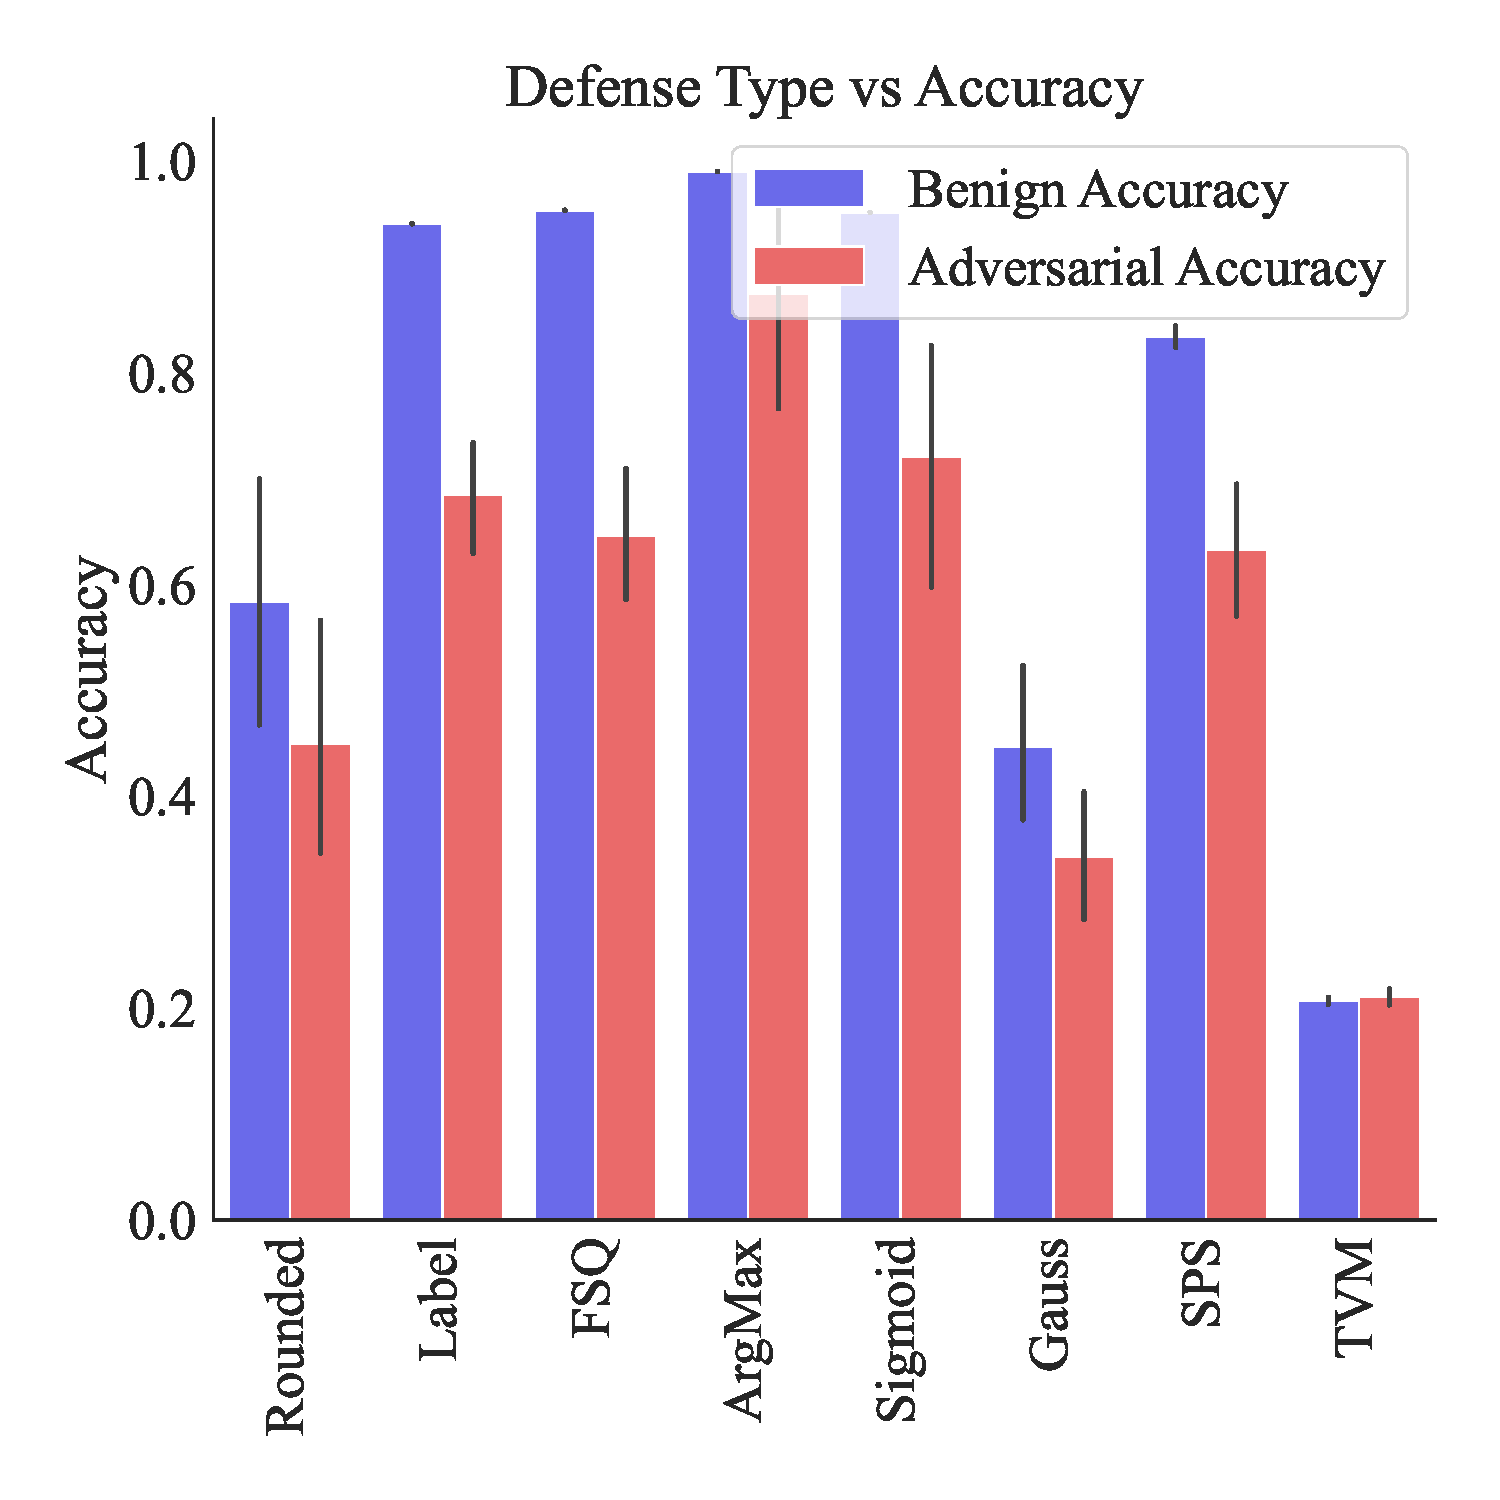
\includegraphics[width=.49\textwidth]{images/cifar-10/def_acc.pdf}
    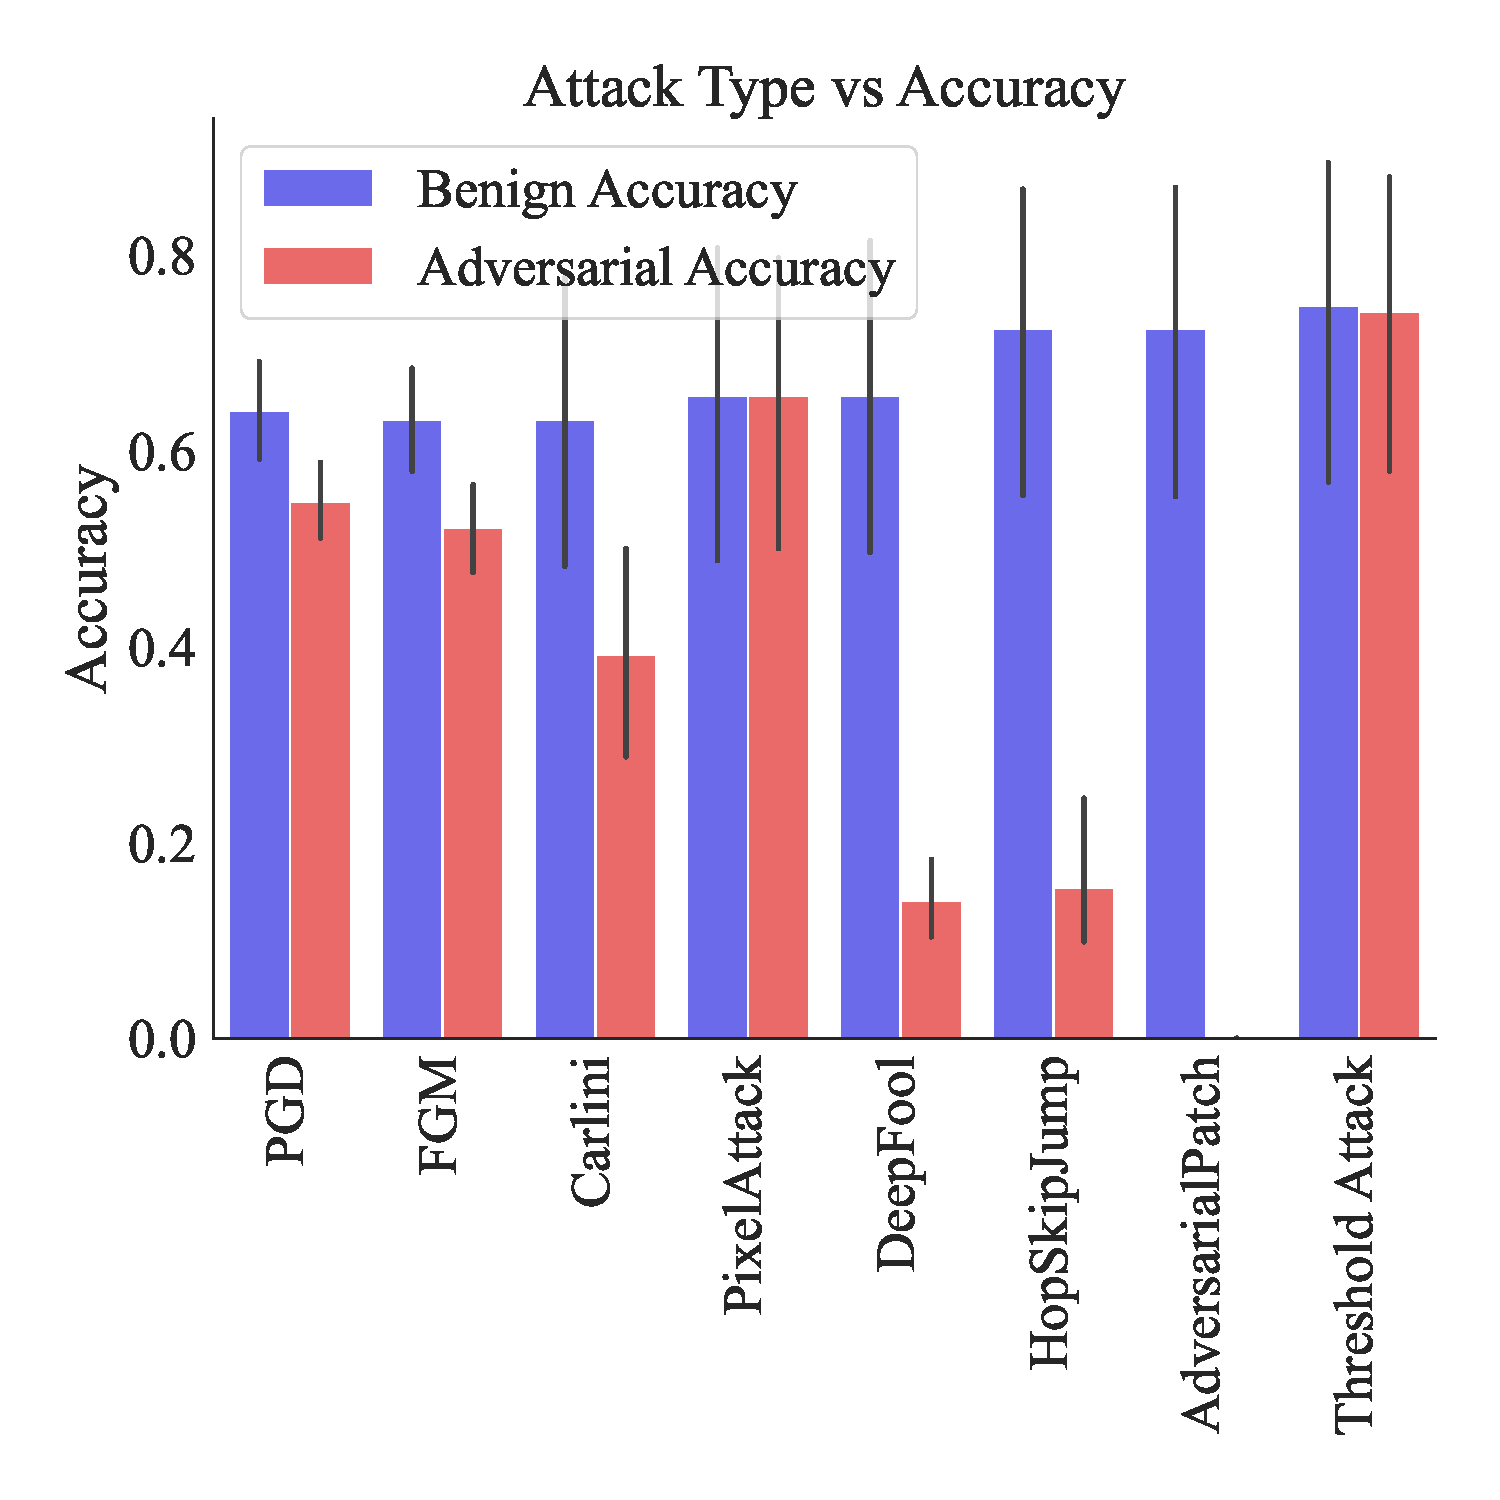
\includegraphics[width=.49\textwidth]{images/cifar-10/atk_acc.pdf}
    \caption{The distribution of adversarial and benign accuracies for each defense (left) and each attack (right). One trial was conducted for each hyper-parameter combination.}
    \label{fig:acc}
    } % end centering
\end{figure}

%% Fit and pred time across defenses and attacks
\begin{figure}[h!]
    {\centering
    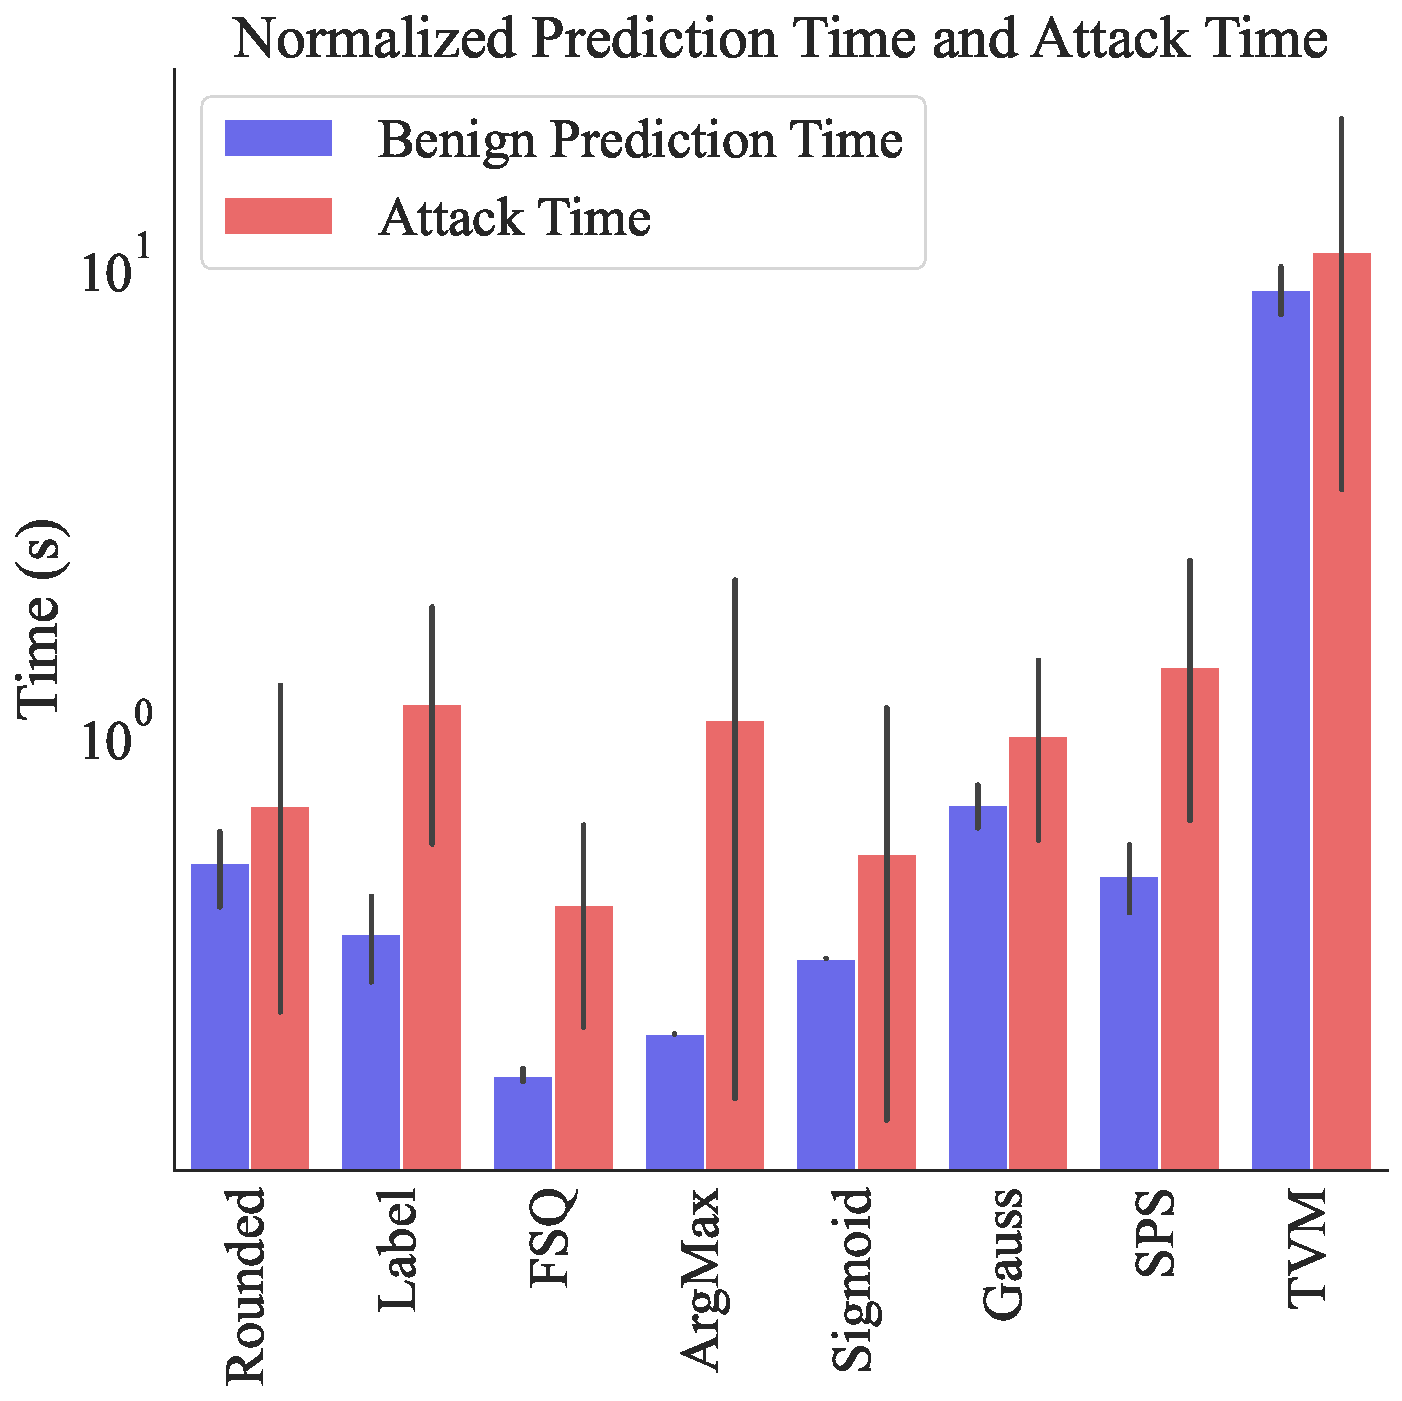
\includegraphics[width=.49\textwidth]{images/cifar-10/fit_time.pdf}
    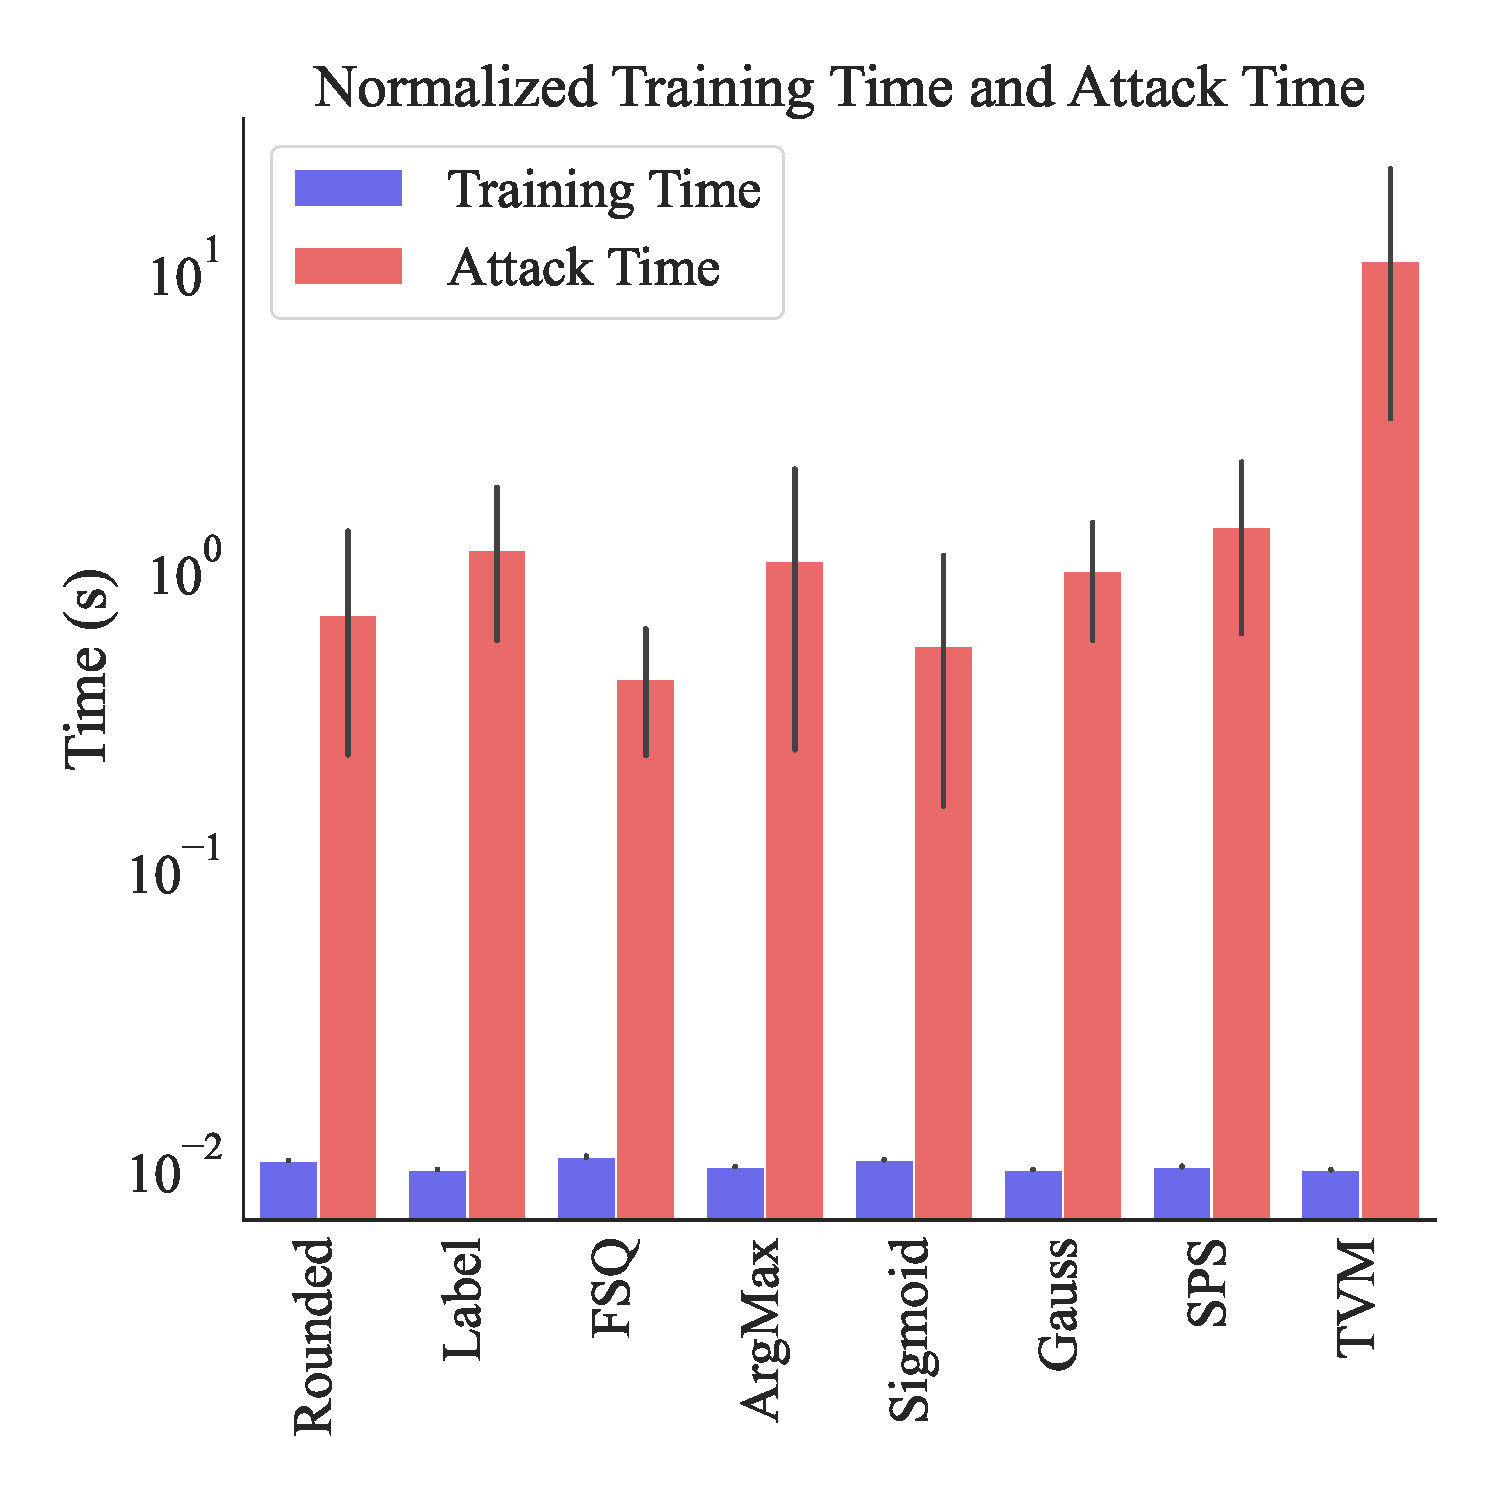
\includegraphics[width=.49\textwidth]{images/cifar-10/pred_time.pdf}
    \caption{The distribution of training times (left) and prediction times (right). Note that adversarial times are identical in each image since fitting and predicting are the same step in this case. One trial is depicted for each hyper-parameter combination.}
    \label{fig:time}
    } % end centering
\end{figure}


%% Failure rate across defenses and attacks
\begin{figure}[h!]
    {\centering
    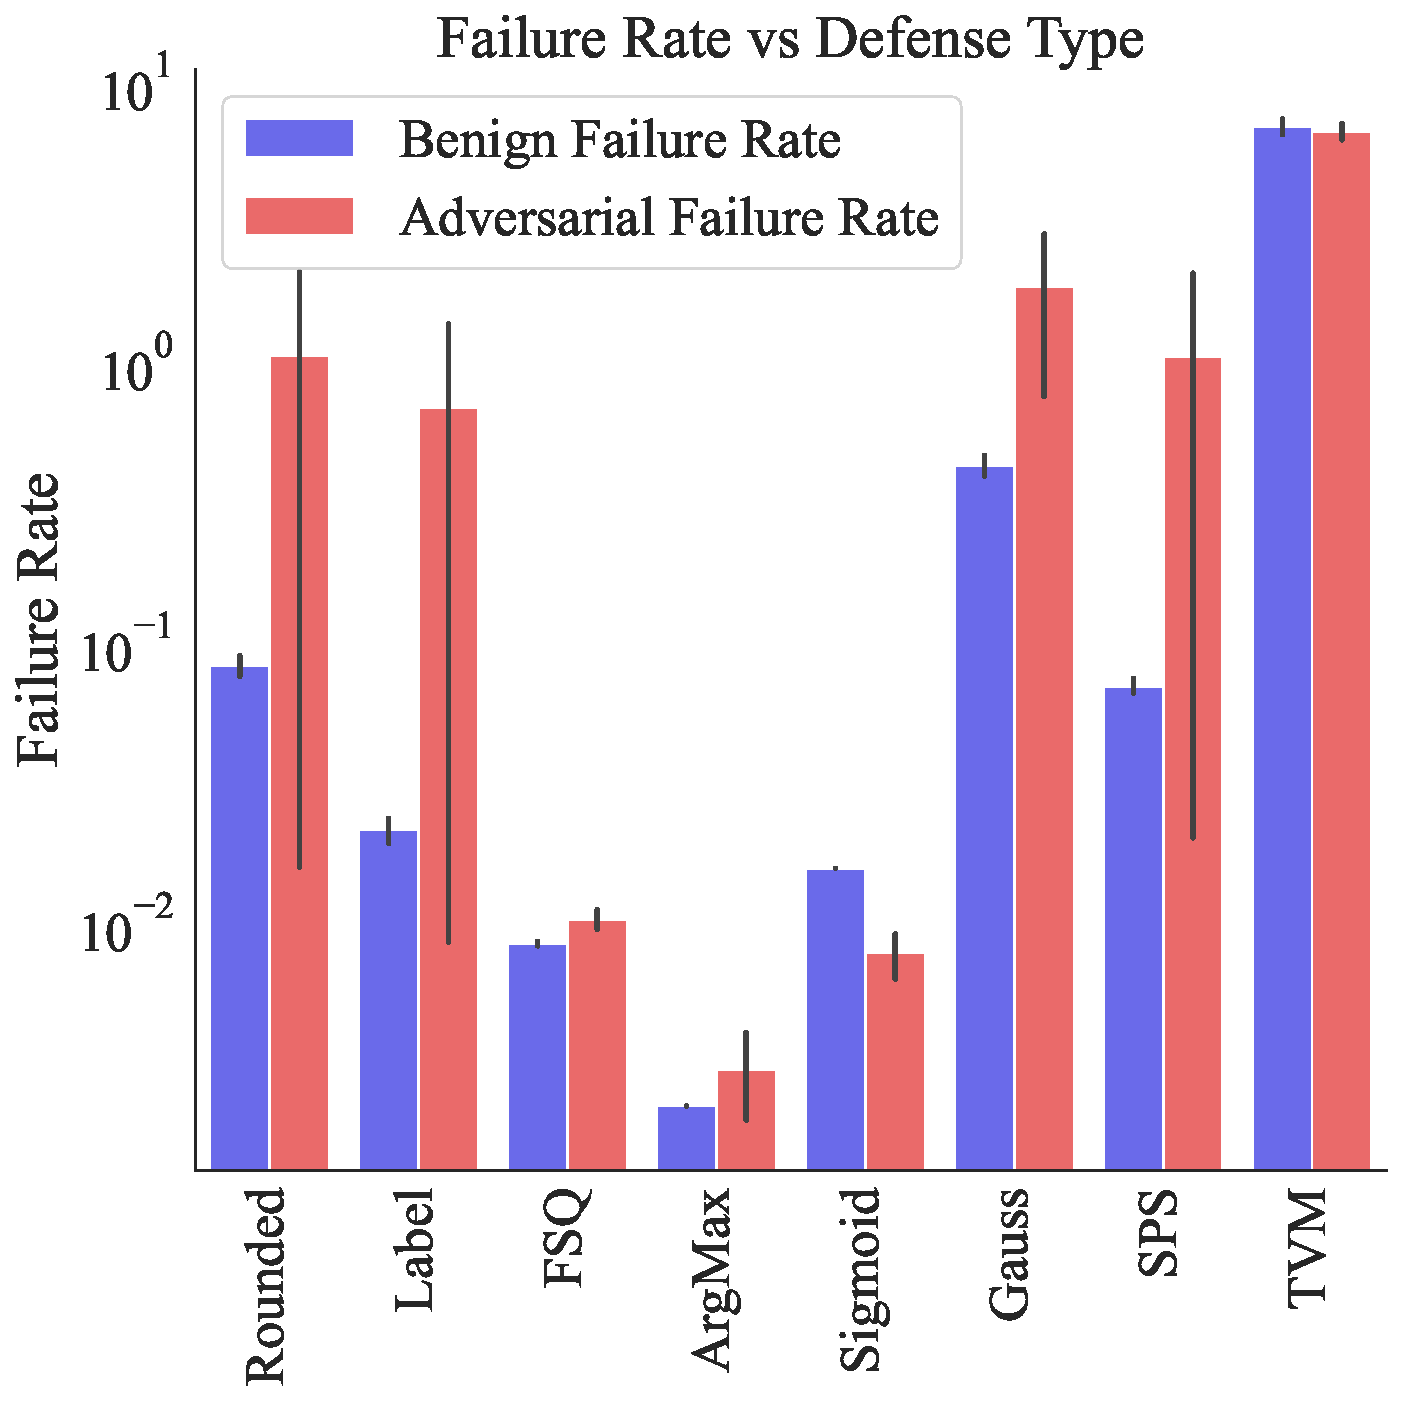
\includegraphics[width=.49\textwidth]{images/cifar-10/def_fail.pdf}
    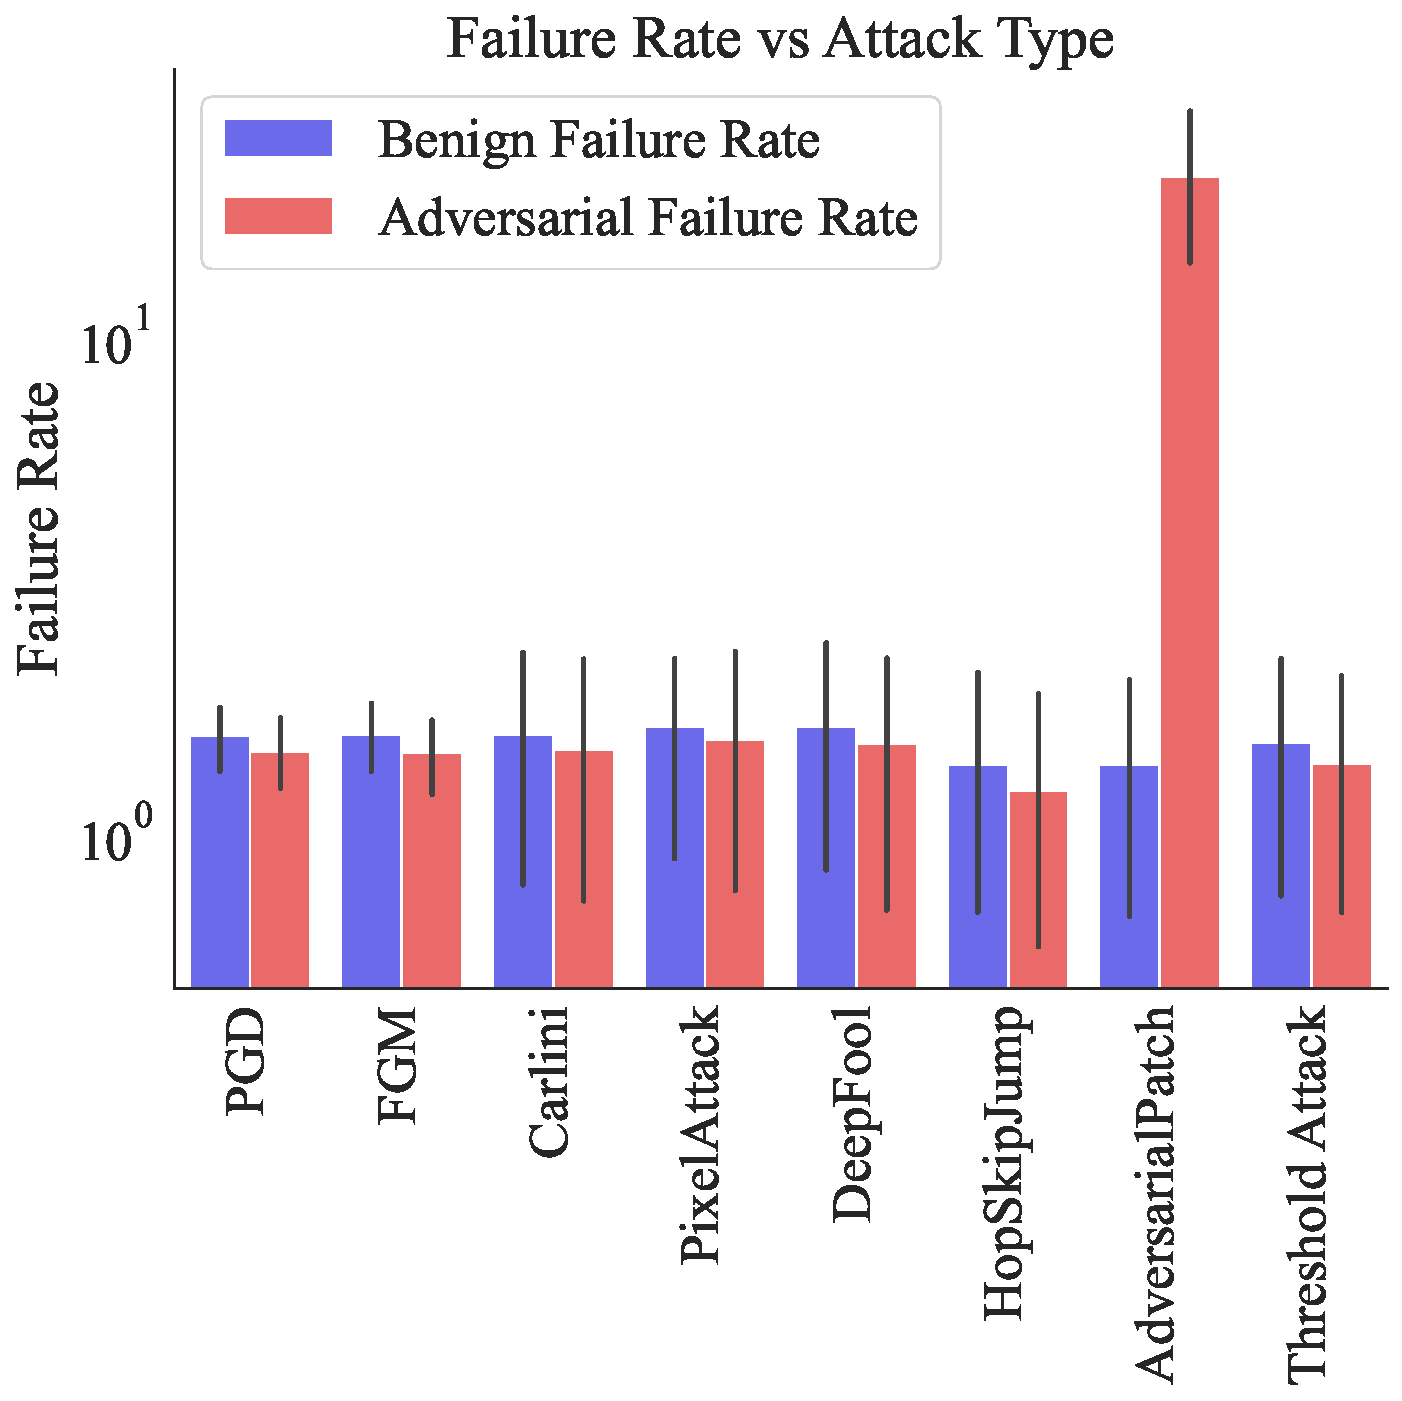
\includegraphics[width=.49\textwidth]{images/cifar-10/atk_fail.pdf}
    \caption{This figure depicts the distribution of failure rates, per defense (left) and and attack (right). This was calculated using Equation \ref{eq:failure_rate} }
    \label{fig:failure_rate}
    } % end centering
\end{figure}

%% Adv Accuracy Grid
\begin{figure}[h!]
    {\centering
    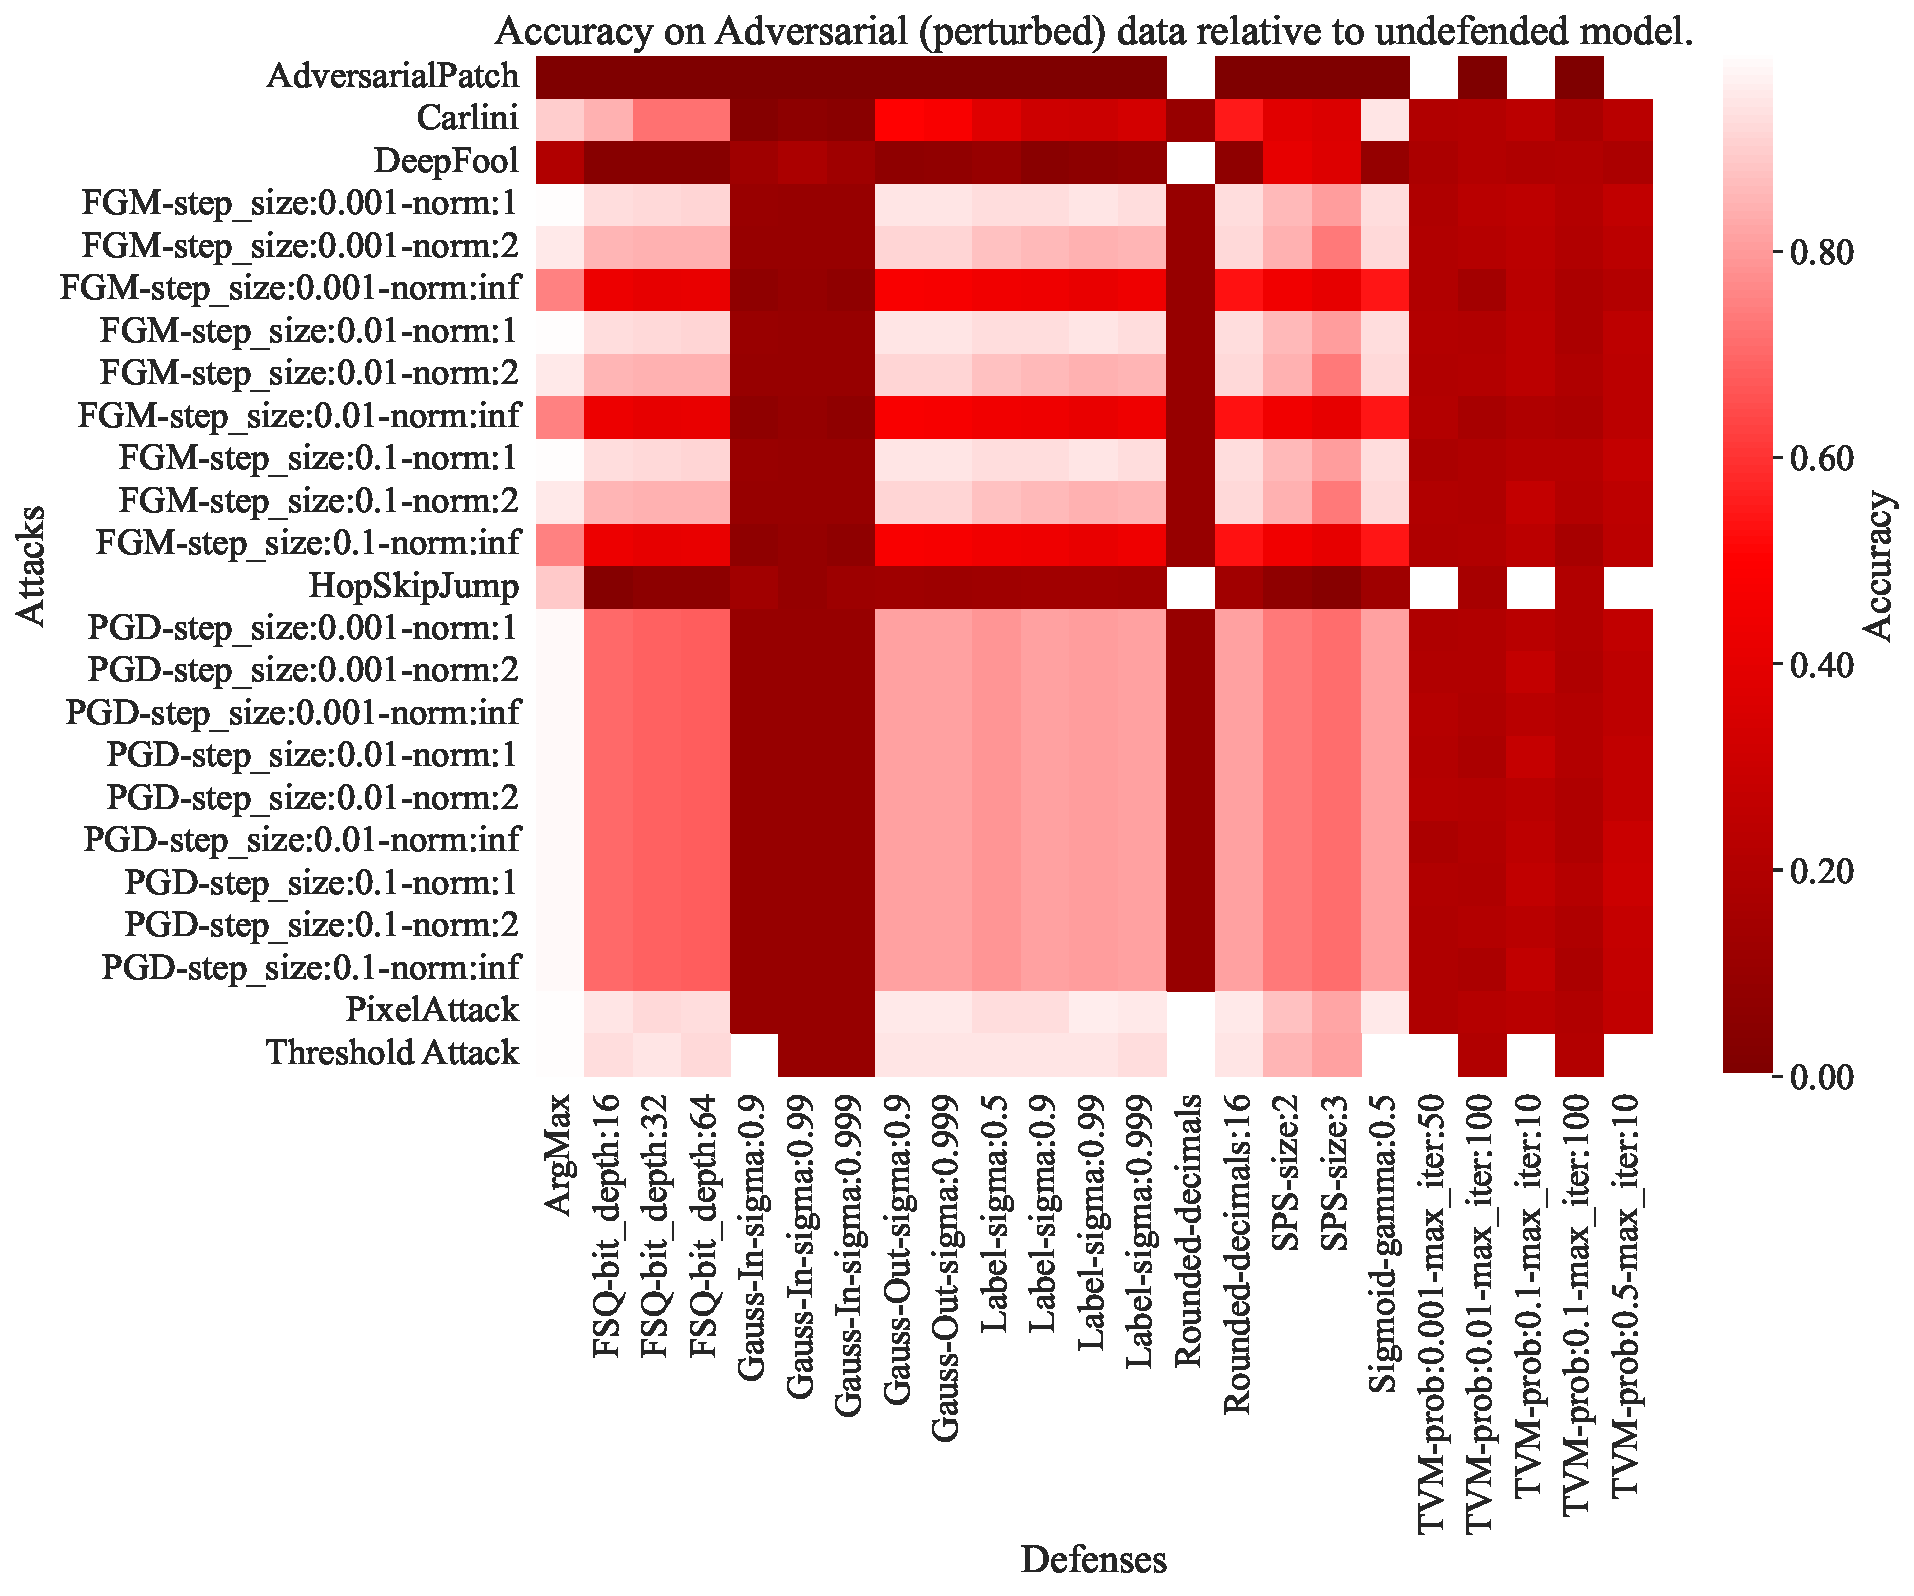
\includegraphics[width=\textwidth]{images/cifar-10/adv_grid.pdf}
    \caption{The adversarial accuracy of each attack against each defense. Blue indicates an improvement relative to the undefended model. Red indicates that defense made a model worse. White indicates no change. Note that no model improves the accuracy score on the original (unpertubed) test set.}
    \label{fig:adv_grid}
    } % end centering
\end{figure}



%% Change Grid
\begin{figure}[h!]
    {\centering
    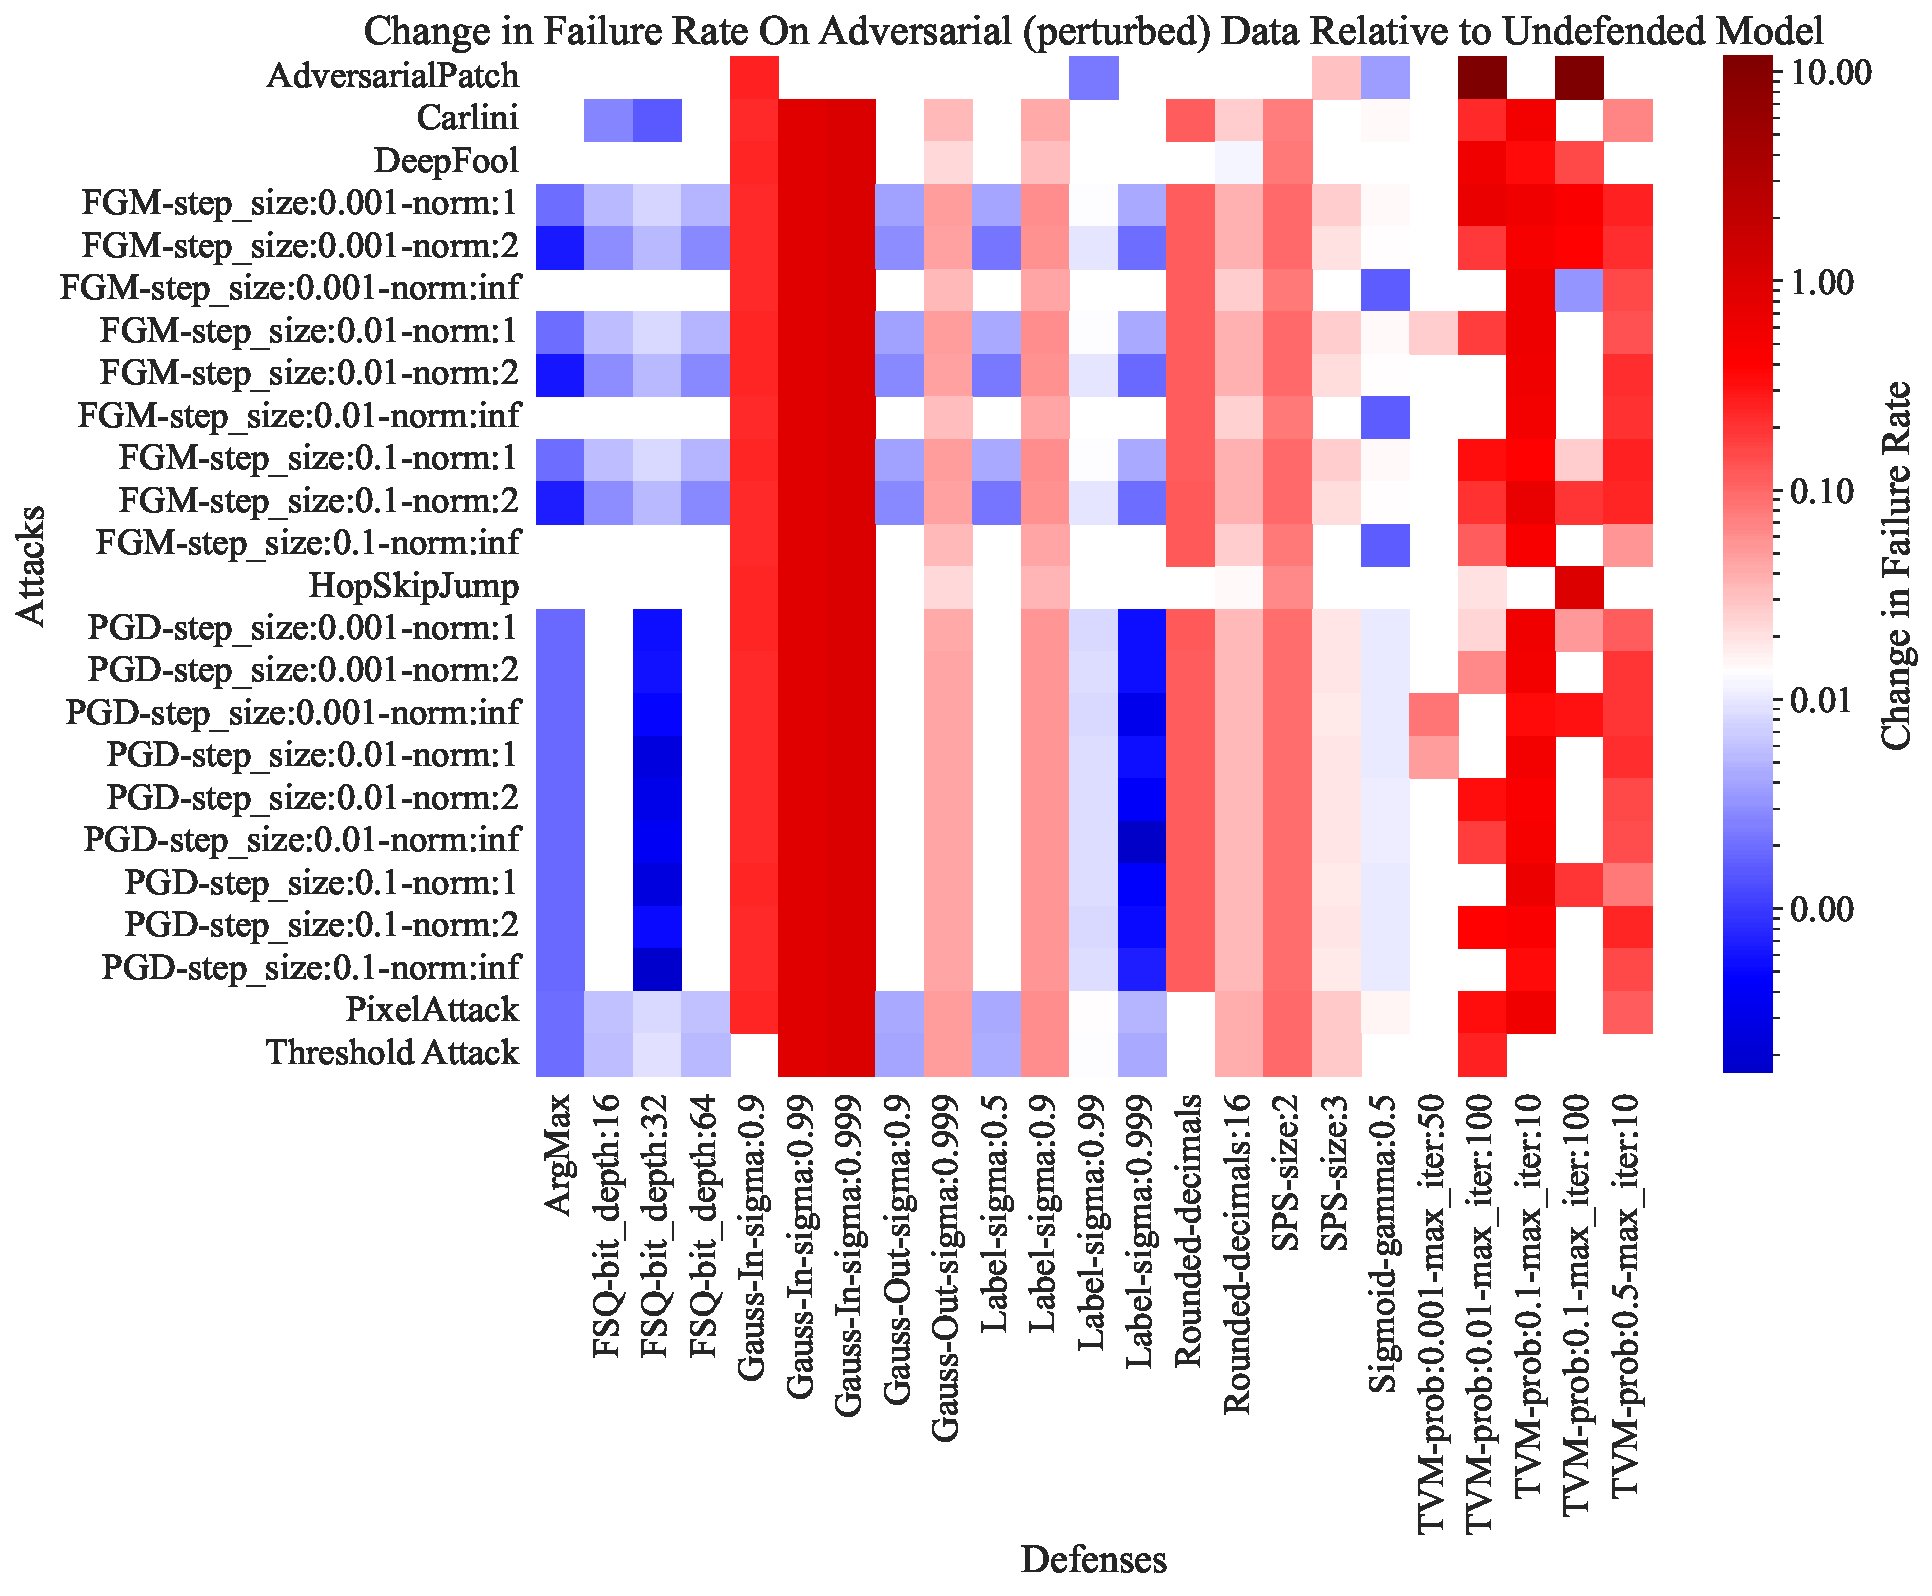
\includegraphics[width=\textwidth]{images/cifar-10/gap_grid.pdf}
    \caption{The change in failure rate between the benign and adversarial cases. Blue indicates an improvement relative to the undefended model. Red indicates that defense made a model worse. White indicates no change. Note that the scale is logarithmic so that marginal gains and substantial losses can be seen clearly.}
    \label{fig:grid}
    } % end centering
\end{figure}






% \section{Discussion}
% \label{discussion}

% \cm{Still integrating the old 'results' section commentary into the discussion. Bare with me since I'm still trying to find the best way to present this information. Some of this only applies to MNIST, but I have since switched to CIFAR and will put MNIST in the appendix since real-world images will be significantly more complex that handwritten black and white numbers with a closed set of possibilities.}

% It is evident that defenses can match the benign accuracy, but the tested defenses never improve the failure rate on the original, unperturbed data 

% From Figure~\ref{fig:acc}, we can see large variations in attack efficacy. Apart from the more `advanced' attacks like DeepFool, HopSkipJump, and Adversarial Patch. However, these take more time to find adversarial examples with. Furthermore, HopSkipJump and Adversarial Patch attacks are not constrained by the perturbation threshold specified for the other attacks. In effect, they can freely replace every pixel of an image, so their nearly-universal efficacy is not surprising.

% As we can clearly see from the dark vertical blue lines in Figure~\ref{fig:accuracy_grid},\tl{Figure reference broken.} certain defenses do appear to increase the strength of the original model (leftmost column). 
    
% The undefended model (control) took the longest time to train (Figure~\ref{fig:trainingtime}),\tl{Figure reference broken.} with spatial smoothing, Gaussian label noise, high confidence thresholding, and the reverse sigmoid output function all reduce model training time.

% As we can see in Figure~\ref{fig:attack_time}\tl{Figure reference broken.}, attacks tend to perform much faster than the original model training (Figure~\ref{train_time}),\tl{Figure reference broken.} with the notable exceptions of the Deepfool and Threshold attacks which sometimes take longer than the original training time.

% Firstly, it is obvious that none of the tested defenses meet even the weakest (\ie $10^{-4}$) safety critical standards. In fact, the only defenses that outperform the control group are Label Smoothing and High Confidence Thresholding which both attempt to enforce a given model to only return outputs when they cross some confidence threshold, with the former happening during pre-processing, and the latter happening during post-processing.

% Notice that this depicts measurements on distinct dataset from the last image, but the benign failure rate and adversarial success rate are more or less identical, hinting at a deep connection between the generalization score (benign accuracy) and the adversarial accuracy.

% We see that each successfully identified frame requires between 10 and 1000 seconds of training with the High confidence, Label Smoothing, and Reverse sigmoid defenses being notable exceptions, logically following their greater adversarial accuracy from above.

% Note that that the time it takes to create a successful attack is much smaller than the time it takes to train on a single image for each defense.

% The time it takes to generate a misclassified adversarial example for each of the attacks. It is evident that all attacks are faster than any given training time. In addition, we see that the advanced attacks like Deepfool, HopSkipJump, and Adversarial Patch are more likely to be successful (Figure~\ref{fig:adv_success_rate}),\tl{Figure reference broken.} this comes with an added computational cost that does not outperform more naive attacks.


% TODO save new images as pdfs, increase label size on the contour map
% htpb, immediately after figures
% h! enforces it to be here

\erik{I  think that a good approach to presenting and discussing results is to, in order: (i) tell is the purpose of the experiment (what you want to evaluate); (ii) what the graph/table/figure is showing (e.g., distribution of adversials, bla, bla, including explaining how the graphs or bars should be read; (iii) what are the general observations; (iv) what are the specific/interesting/unexpected observations; (v) what are the conclusions from the experiments (ideally answering (i). In your first paragraph below, you basically jump directly to (iv). The headline "Benign vs. Adversial Accuracy" partly serves the purpose of (i), but you never use these terms in the text so the headline becomes somewhat detached. (One sentence to explain the two terms would also be good for completeness, despite known to the readers from the field.) The explanation of how to read the bars can be given as part of the legend or caption in the figure, but the other parts are better done in the text. (As a guiding message, the whole story should be in the text and the figures should support the story but not replace it.)}


\paragraph{Benign vs Adversarial Accuracy.}
Figure~\ref{fig:acc} depicts the distribution of adversarial and benign accuracy, as calculated by Equation~\ref{eq:accuracy}.
From the rather large 95\% confidence region, we see that both attack and defense hyper-parameter tuning have significant effects on the accuracy of a given method. Figure~\ref{fig:adv_grid} depicts how adversarial accuracy differs from the benign accuracy, broken down for each attack and defense combination.  We see that, for every defense, that adversarial accuracy is lower than benign accuracy, confirming the accuracy vs robustness trad-off mentioned in the literature. The tested defenses each attempt to strategically destroy, smooth, or average data in the original dataset or during the output phase of the model, which results in a loss of precision that makes the benign accuracy worse. Furthermore, when we examine the attacks in Figure~\ref{fig:acc}, we see that Deepfool, HopskipJump, Carlini, and Adversarial Patch are able to confuse the model more that half of the time. It shows that most defenses have little to no effect on the failure rate of the underlying model. The notable exceptions to this are the label smoothing defense which has a tendency to mislabel images that are not prototypical and the feature squeezing defense when the bit depth is reduced to 4, effectively destroying half of the information in the 8-bit images. When we examine failure rate against various attacks, we see that a clever choice of hyper-parameters is critical to a successful gradient descent attack whereas the more `advanced' techniques are more consistently successful at evading the various defenses in a way that does not require tuning.


\paragraph{Computational Cost.}
Figure~\ref{fig:time} illustrates the essential problem of adversarial defense, wherein it is consistently faster to break a model than it is to build it. In order to control for computational cost, we measured each time as a process time, reducing the jitter due to operating system operations and shared kernel constraints. We see that defenses require between 1 and 100 seconds of training per success, broken down by defense in Figure~\ref{fig:time}. However, attacks (see Figure~\ref{fig:time}) require as few as $10^{-5}$ seconds in the worst case and $10^{-1}$ seconds if the attacker is poorly tuned to the model, with the average attack time falling after around $10^{-5}$ seconds. Furthermore, we see how various defenses manage the trade-off between computational complexity and efficacy, with only the feature squeezing and augmentation defenses significantly improving over the control model. Total variance minimization creates models that train quickly, but perform poorly so this rate is overly optimistic. When we combine the data from Figures~\ref{fig:acc} and~\ref{fig:failure_rate} with the failure rate Equation~\ref{eq:failure_rate}, we produce Figure~\ref{fig:failure_rate}. We see what the


\paragraph{Images as Noisy Channels.}
Figure~\ref{fig:grid} depicts how each defense fares against each attack. We see that the control group (Argmax) is fairly successful, even when compared to a large set of defenses. Furthermore,  Notice that the feature squeezing defense with a bit-depth of eight performs the best, which reflects the fact that our images are originally 8-bit and that casting them to a 64-bit floating-point number in Python works against our goals. There were nearly identical results for the High Confidence defense, which even outperforms  the control against DeepFool, one of the consistently strongest attacks (see: Figure~\ref{fig:acc}). However, the HopSkipJump and Adversarial patch attacks, which  are not constrained by perturbation distance consistently evade every defense. This is expected as our adversarial patch attack has no constraints and can effectively replace every pixel in an image and the HopSkipJump attack avoids decision boundary obfuscation by perturbing an image by an unconstrained amount, restricted only to the total number of queries (ten in our case).


% \paragraph{Failure Rate}
% Furthermore, the distributions of these two measures are nearly identical, hinting at a deep topological connection between a model's ability to generalize beyond the training data and its ability to successfully defend against an intentional adversary.








\section{Conclusion}


Neural networks are being deployed in a wide variety of industrial applications with real-world safety considerations, that despite high accuracy scores, fail against a wide variety of attacks that overwhelmingly require fewer computational resources than building the original model. While `weak' attacks are fast, they require hyper-parameter tuning and retrospective evaluations that make them less effective, but nonetheless cheap-enough to execute (especially if our attacker has access to a distributed network via a botnet or malicious browser exploit). The efficacy of even single-byte attacks against otherwise very accurate models raises questions not only about the intentional adversary, but also how a system will handle real-world, `legitimate' anomalies like dust, lens aberration, and sensor failure. When we consider the strongest attack, DeepFool, we see that 80\% of all samples are corruptible under our meager one-byte distance constraint. When we remove this distance constraint, we find that nearly every sample can be fooled with the addition of an adversarial `patch' on the original image (Figure~\ref{fig:grid}) even when we constrain our algorithm to a small number of iterations ($\leq 10$). That is, if we assume that our attacker has an unlimited budget, we cannot even hope to defend against these attacks.

Furthermore, since this failure rate is based on process time, it is obvious that more powerful hardware, without underlying changes to the model architecture, would result in a larger failure rate since we merely fail to meet our goals faster. That is to say, these problems are inherent to the model and not something that we can solve with more processor cycles. Furthermore, even when we obscure everything from the user except model output, we can consistently break models in as few as ten queries to the obfuscated API (\ie HopSkipJump atack). We found that adding Gaussian noise to the model outputs or training images, reducing the bit-depth of the numerical calculations to match the precision of the image, and setting a confidence threshold were marginally effective defenses when compared to the control model. However, none of these defenses reach the regulatory standards required for safety-critical systems; in fact, they fail by several orders of magnitude. Furthermore, any gains seen in the failure rate (Figure~\ref{fig:grid}) are inconsistent while universally reducing the accuracy on the original (unperturbed/benign) data (Figure~\ref{fig:acc}).

If we use this better hardware to process more images during training, the accuracy improves as $\mathcal{O}(1/\sqrt{n})$ \cite{vapnik1994measuring} while the costs of such accuracy scale linearly with the number of samples. These extra bits of precision are unlikely to solve the robustness problem as they merely expose more bits to the attacker with each query. Because adversarial accuracy is tightly coupled to benign accuracy and the ability for a model to generalize (see Figures~\ref{fig:failure_rate}, improving the benign accuracy seems to penalize the adversarial accuracy by the same degree. That is, more accurate models tend to be more vulnerable to small perturbations of the input since each query reveals more `useful' bits to the attacker. 

Furthermore, because attacks are generally easier to generate than models (as measured by input samples, queries, or processing time), we must question the real-world efficacy of any system that relies on these networks to make predictions that meet the legal standards that define `safe.' 

% Motivation
% Restate Problem
% Restate methods
% Restate contributions
% Restate conclusion
%TODO: https://arxiv.org/abs/1804.05296


\bibliographystyle{plain}
\tl{The arXiv references don't need to have the arXiv identifier twice. The first reference only give the initials of the authors, while all other references have the full names.}
\tl{Add authors and publishers, or in case of web pages visit dates and URLs, to the Traffic safety facts and Iso standard.}
\tl{References 27 and 28 are the same. Pick one and use that one.}
\tl{References 1, 2, 26, 37, and 45 need more information to be found.}
\bibliography{bibliography}
\end{document}
